\documentclass[a4paper,10pt]{report}
\usepackage[utf8]{inputenc}
\input{/home/andi/Studium/LaTex/preambel.tex}


%opening
\title{Magnetic Excitations In Iridates}
\author{Andreas Karl Leonhardt}

\begin{document}

%\maketitle

\begin{abstract}
In this thesis we investigate magnetic properties of Iridates, 
compounds that contain orthorombic Iridium and can be described by the Hubbard model for effective spins.
We use a mean-field approach to calculate the dynaimc magnetic susceptibility for certain components.
They are compared to measurements and other models, mainly Heisenberg models. 

We found the Hubbard model with up to third-neighbour interactions to provide results that agree well with experiment.
% U as only free parameter
%quantum corrections
\end{abstract}

% ABSTRACT IN NORWEGIAN??? 

\tableofcontents

\chapter{Introduction}

% remember: there will be an abstract, that contains some introdcutory blabla.
Iridates is the name for a group of anorganical chemical compounds that contain oxydized Iridium.

% interesting examples here
These materials gained a lot of attention in the last decade due to their variety of interesting configurations.
Due to their configuration of an Iridium ion surround by several oxygen anions, they can be described as effective spin systems.
Therefore they are a realization of interesting theretical models such as the Hubbard and the Heisenberg model.
Some of the compounds have a layered structure, leading to low-dimensional systems.


Iridates share a lot of properties with the cuprates. 
Ever since high temperature superconductivity (HTSC) was discovered in cuprates, 
they were intensively investigated. 
Due to the chemical similarity of irdium to copper, it is possible to create materials that share the same geometry as the ones known from cuprates.
Replacing copper with irdium yields interesting effects due to their physical differneces.
The higher charge of the iridium nucleus for example enhances the spin-orbit coupling in the active orbitals.
This creates interesting new effects when embedded in a pervoskite structure, as it is the case in the iridates.
%
% same shit, different try
%
Iridium and Copper have similar chemical properties. 
Iridates are therefore quite similar to Cuprates. 
The later one are intensively investigated ever since high temperature superconductivity was first realized in doped cuprates in 1986 \cite{}.
Both are strongly interacting, which makes them a Mott-insulator at half filling.
Since Iridium is a heavier element some of the parameters are different for Iridates. 
Due to the larger charge of the nucleus, spin-orbit coupling (SOC) is enhanced in Iridates compared to cuprates.
This creates new effects and changes the macroscopic behaviour. 
We find Iridates that behave like soin$\frac12$ systems with half filled bands. 


%They are promising candidates to provide a realization of theoretical models.

The term was coined in resemblance of cuprates, a similar group of materials with Copper instead of Iridium.
% However, both terms are not strictly defined and may include some exceptions with non-ionic bounds.
Cuprates are intensively investigated since the 1980s, when high temperature superconductivity was first realized in Cuprates.


Here we refer to a certain subclass of these materials, where ions of Iridium and Copper respectively are embedded in an octahedral of oxygen ions.
Depending on their geometries, these materials show a wide range of interesting effects.
They provide a realization of two-dimensional spin systems with strong interactions. 

% some words on cuprates and high temperature superconductivity
% similarity to Iridates
% differences in Iridates
% first experimental realization of Iridates. 
% Further specialization on materials investigated here.

% it is insulating, unexpected, compare to cuprates


We find realizations of low-dimensional spin systems

The research on Iridates, both experimentally and theoretically, became an area of intesiv research in the recent years. 
Their share a lot of features with the Cuprates, since Iridium and Copper are almost identical in their chemical properties. 

However, since Iridium is a heavier element, its compounds show new features that differ from the ones known from cuprates.
The most interesting effect is the enhanced spin-orbit coupling due to the heavier nucleus.
By this, the replacement of Copper by Iridium might have drastic on the macroscopic behaviour. 
One example is a transition from the conductor to an Mott-insulator in Sr$_2$XO$_4$, 

Depending on the orientation of these octahedrals, the number of oxygen ions shared between two octahedrals varies for different materials. 





\section{Motivation}

% Why are Iridates interesting
% - similar to Cuprates, and they pffer a variety of materials with interesting properties, such as HTSC. 
% - - similar chemical configuration, but higher Z lead to :
% - - stronger Spin-Orbit coupling might introduce new effects. (\lambda \propto Z^4)
% - geometric structure: layered and therefore effective 2D systems (pervoskite)
% -- pervoskite structure and SOC create effective spin-$\frac12$ systems
% -- different geometries of spin sites: rectangular, triangular, realization of Kitaev Model.
% -outline doping?
% theoretical point of view: Playground for Hubbard model


% approach outline: 
% -Describe as spin system
% -treat in mean-field approach (taken from cuprates)
% -calculate observables and compare to experiment for specific material(s)
% -determine parameters of model (basically U)
% - show that this is a reasonable approach worth for further usage.
% -compare models: Hubbard vs. Heisenberg, 
%  -or since Hubbard $\stackrel{U\rightarrow }infty}{\longrightarrow}$ Heisenberg, is Heisenberg sufficient, valid, good?
% - find ground state: Mott insulator vs … ? 

% What could be done with that? 
% engineering of Kitaev model & other stuff?
% HTSC for doped Iridates?

% controversy about:
% -Mott insulator (paper) (see above)
% -parameters, especially U
% -if HTSC is possible
% need better unterstanding in general blabla.



\section{Outline \& Goals}

First the characteristic configuration of the crystal is  investigated.
We will see, how Iridium embedded in an octahedral of oxygen ions  with strong  SOC
creates states with an effective total angular momentum of $J=\frac32$ and $J=\frac12$.
While all $j=\frac32$- states are occupied, the later ones are half filled in the case of an undoped material.
They form the active band, which allows us in a tight binding approximation to proceed to a pure spin model. 
As a strongly correlated system it can be described with the Hubbard model. 
This is the easiest way of including interactions in a spin system.
% $t-U$ and $t-t^{\prime}-t^{\prime \prime}-U$


We then solve the Hubbard model in the mean-field approach.
The goal is to calculate the dynamical magnetic susceptibility.
From this we can extract the spin wave dispersion, which 
can be directly compared to results from neutron and X-Ray scattering experiments.
We follow the calculation scheme by XXYY \ref{cuprate paper} that was used for the cuprate LaCuO in 19XX.\todo{name, reference, material and year}

The actual calculations will be performed in the large U limit and compared to the Heisenberg model.
Since the Heisenberg model can be dervied from the Hubbard model in this limit, we can use this to validate the calculations.
We calculate the dispersion with parameters from Sr$_2$IrO$_4$ for different band structures.
The results were compared to measurements on this material. 
The interaction parameter $U$ is the only adjustable parameter and will be fitted to give the best match to observations.
We want to show that the approach outlined above provides results that agree well with measurements and is capable of reproducing the main features of the dispersion. 
%
% necessity of t-t'-t''?


  

\chapter{Towards A Spin Hamiltonian}

\section{Iridates}
% proper definition of iridates
Iridium is one of the rarest metals on earth and highly corrision-resistant. 
It belongs to the transition metals, i.e. it has a only partially filled $d$ shell.  
The shell structure of atomic iridium is given by $[\mathrm{Xe}]4f^{14}5d^7 6s^2$.
% ${\mathrm{Sr}}_{2}{\mathrm{IrO}}_{4}$
In compunds it can be found in different oxidation states, ranging from -3 to +6.
In the compounds treated in this thesis iridium is fourfold oxidized to $\mathrm{Ir}^{4+}$, 
which removes the $6s^2$ electrons as well as two electrons from the $5d$ shell. 
The outermost shell is therefore a the half-filled $5d$ shell ~\cite{Abragam70}.


%(the ion shell structure does not follow the Aufbau principle. 
%Therefore has $\mathrm{Ir}^{4+}$ a different shell structure than Tantalum, even though they have the same number of electrons. 
%This is because of the different charge of the nucleus, that leads to a greater seperation in energs levels with different quantum number n ($\propto \frac{Z}{n^2}$)).

The other elements of the compunds treated in this thesis are oxygen and rare earth metals. 
The oxygen is two fold ionized and has therefore only the closed shells $1s^2,2s^2,2p^6$.
The same hold for the rare earth metals, strontium is reduced to 
$\mathrm{Sr}^{2+}$ with the electron configuration of $\mathrm{Kr}$. 
Both the rare earth metal and oxygen have therefore zero total angular momentum and spin. 

Iridates show a great variety of geometrical configurations. 
We will focus on Sr$_2$IrO$_4$, which is part of the Ruddelson-Popper series of Iridium oxides, Sr$_{n+1}$Ir$_{n}$O$_{3n+1}$ with $n =1$. 
Other possible values are 2 and $\infty$.
Sr$_2$IrO$_4$ has the structure of a layered perovskite, that means it consists of layer with a structure similar to CaTiO$_3$.
The later one is also called perovskite and lends this type of configuration its name.
The main feature of the pervoskites is one ion, in this case Ir$^{+4}$  embedded in an octahedral of oxygen ions.
The octahedra itself are situated on a square lattice, whith the oxygen ions on the face senters,
while the rare earth metal contributes to the relative orientation of the octahedra. 
%
In the case of Sr$_2$IrO$_4$ the octahedra share corners in the $x$-$y$-direction, while beeing separated by a Sr$^{2+}$ ion in the z-direction.
Due to a shift between two subsequent layers, the square unit cell consists of two layers. 
An octaheder of one layer matches an Sr ion of the other, perventing thereby corner sharing in the $z$-direction and yielding the separation of layers. 
%
Furthermore, the octahedra are tilted in a staggered pattern by $\Theta = \pm 11^{\circ}$ \cite{PhysRevB.49.9198}.
This enlarges the cubic unit cell to $\sqrt2 a\times\sqrt 2b \times 2c$.
In $x$- and $y$-direction we have to take the diagonal translation vectors, while we get 4 layers in $z$-direction, until we reach the same pattern again. 
%
We will neglect the rotations in proceeding to an model of effective spins, but regain the influences it has on the magnetic structure in the final interpretation of 
measurable quantities. It shows that these rotations provide an explanation for a small ferromagnetic moment in an otherwise antiferromagnetic material. 
\todo{picture of Sr2IrO4 unit cell, take from \cite{PhysRevLett.108.177003} if needed}

\subsubsection{Ligand Field}

The $5d$ states  in a free iridium ion are degenerate due to rotational symmetry of the atomic Hamiltonian. 
We represent them by the states $x^2-y^2,z^2,xy,xz,yz$, which are related to the spherical harmonics $Y^2_m$ for $m=0,\pm1,\pm2$ by a unitarian transformation.
As such, they all have angular momentum l=2. 
and they form an irreducible representation of the rotation group.
\begin{center}
\begin{tabular}{|c|c|c|}
 \hline
 $xy$ & $\frac{\im}{\sqrt 2} \left( Y^{-2}_2 - Y^2_2 \right)$ & $\sqrt{\frac{15}{4\pi}} \frac{xy}{r^2}$ \\
 $xz$ & $\frac{  1}{\sqrt 2} \left( Y^{-1}_2 - Y^1_2 \right)$ & $\sqrt{\frac{15}{4\pi}} \frac{xz}{r^2}$ \\
 $yz$ & $\frac{\im}{\sqrt 2} \left( Y^{-1}_2 + Y^1_2 \right)$ & $\sqrt{\frac{15}{4\pi}} \frac{yz}{r^2}$ \\
 $z^2$& $ Y^0_{2} 					      $	& $\sqrt{\frac{15}{4\pi}} \frac{3z^2-r^2}{2r^2\sqrt 3} $\\
 $x^2-y^2$&$\frac1{\sqrt 2} \left( Y^{-2}_2 + Y^2_2 \right) $ & $\sqrt{\frac{15}{4\pi}} \frac{x^2-y^2}{2r^2} $ \\
 \hline
\end{tabular}
\end{center}
%
Embedding the ion in a crystal breaks the rotational symmetry and the degeneracy of these states will be lifted.
Since the ion is now surrounded by oxygen ions, the so calles ligands, in the form of an octahedron, the 
full rotational symmetry is reduced.
Due to the geometry of the ligands, the poential is symmetric under transformations, that map an octahedron or equally a cube on itself.
These transformation build the group $O_h$.
Comparing the characters of the irreducible presentations for the $O_h$ group with the ones for for the full rotation group, we find that 
the later one has to split up into two subgroups, 
the three-fold degenerate $t_2g$ states consisting of the $xy,xz,yz$ orbitals and the two-fold degenerate $e_g$ states $z^2$ and $x^2-y^2$ \cite[p.70 et sqq.]{Tinkham64} 
% this is just a very short outline, can, but doesn't need to be explained further.
% in the latter case, a nice reference woudn't hurt.
Group theory alone does not provide the energtic order of this two subgroups. 
From … \todo{where} we know, that the $e_g$ states correspond to a higher energy level.
For a strong crystal field, as we have in these materials, the $e_g$ states are well above the Fermi level and are therefore unpopulated,
in contrast to a weak crystal field, where orbitals are filled according to Hund's rule. 
For iridium we deal with the $5d$ states, which are more extended than $4d$ and $3d$ states. 
This reduces the repulsion between eletrons, which further helps favouring double occupancies in the $t_{2g}$ over filling the $e_g$ states.
Finally, the $t_{2g}$-states contain all 5 electrons belonging to the $d$-shell.
The $xy,yz,xz$ states build have an effective angular momentum of $L=1$.




\section{Strong Spin-Orbit Coupling}


Until now we neglected interactions between angular momentum and spin. 
The coupling $\lambda$ of total angular momentum $L$ and total Spin $S$ is proportional to the charge of the nucleus in 4th power, $Z^4$.
Spin orbit coupling (SOC) is therefore more important in heavier elements and not negligible in iridates.
Strong SOC is the main difference compared to the cuprates, which have a very similar structure otherwise.
It is the reason for interesting new effects like the insulating behaviour up to high temperatures. 

We introduce SOC by adding the term $\lambda \sum_{i} \hat{\vec L} \cdot \hat{\vec S}$ to the Hamiltonian.

%
% tight binding before that?
%
% How to introduce band structure, without introducing it twice?
% qualitative description here, calculation later, or even in appendix?
%
% go through the stuff down there.

% First: picking out some parts that are ready to send !!!!!!!!!!!!!!!!


for LS-coupling: 
\cite{PhysRevLett.105.216410}


In the $5d$ elements spin orbit coupling (SOC) plays an important role since it increases with the charge of the nucleus.
\todo{theoretical background for string SOC according to Z.}
Since there is one hole in the $t_{2g}$ shell left, the total Spin is $S=\frac12$. 
When coupled to the effective spin $L=1$ as mentioned above, 
the sixfold degenerate $t_{2g}$ states (including spin degeneracy) split into a fourfold degenereate level with $J=\frac32$
and twofold degenerate level with $J=\frac12$. The latter one is higher in energy, since we couple an \emph{effective} angular momentum to the spin,
thus the paralell coupling is energetically favourable.
In the ground state the $J=\frac32$ band will be filled, while the $J=\frac12$ band is half filled, leaving us with an effective Spin$\frac12$ system on each Iridium site in the grid.
\todo{create/include graph similar to \cite{PhysRevLett.101.076402}}

The two states are given by a linear combination of the molecular orbits and spin states,
\begin{equation}
 \ket{J_{\mathrm{eff}} =\frac12, M_{J_{\mathrm{eff}}}= \pm \frac12}
 = 
 \frac{1}{\sqrt{3}} \left( \ket{yz,\pm \sigma} \mp \im \ket{zx,\pm \sigma} \mp \ket{xy,\mp \sigma} \right).
\end{equation}
where $+\sigma = \uparrow, -\sigma = \downarrow$. The moelcular orbits are given by linear combinations of the spherical harmonics
\begin{IEEEeqnarray}{rCl}
\ket{xz} &=& \frac{1}{\sqrt{2}} \left( Y_2^{-1} - Y_2^{1} \right) \\
\ket{yz} &=& \frac{\im}{\sqrt{2}} \left( Y_2^{-1} + Y_2^{1} \right) \\
\ket{xy} &=& \frac{\im}{\sqrt{2}} \left( Y_2^{-2} - Y_2^{2} \right) 
\end{IEEEeqnarray}

\todo{transformation properties of the ground state}

%%%%%%%%%%%%%%%%%%%%%%%%%%%%%%%%%%%%%%%%%%%%%%%%%%%%%%%%%%%%%%%%%%%%%%%%%%%%%%%%%%%%%%%%%%%%%%%%%%%%%%%%%%%%%%%%%%%%%%%%%%%%%%%%%%%%%%%%%%%%%%%%%%%%%%%%%%%%%%%%%%%%%%%
\section{Spin System And The Hubbard Model}

\subsubsection{Tight Binding Model} % in second quantization




Energy eigenstates of the crystal must be Bloch states, defined by  the relation
\begin{equation}
 \Psi_{n,\vec{k}} \left( \vec{r}+\vec{t}\right) = \euler^{\im \vec{t} \vec{k} } u_{n,\vec{k}} \left( \vec{r} \right), \label{BlochDef}
\end{equation}
where $\vec{t}$ denotes a translation vector of the lattice, e.g. one that leaves the lattice unchanged, 
and $u_{n,\vec{k}}$ is a periodic function with the same periodicity than the lattice.
Using a Fourier transform on the Bloch states of different bands $n$, we get the so called Wannier states,
\begin{equation}
 \Psi_{\vec{R}_i, n} \left( \vec{r} \right) = \frac1{\sqrt{N}} \sum_{\vec{k}} \euler^{\im \vec{k}\vec{R}_i } \Psi_{\vec{k}, n} 
\end{equation}
Those are no longer eigenstates of the Hamiltonian, but still orthonormal, since the transformation is unitarian. 
Furthermore they are localized around the positions $\vec{R}_i$.
Instead of the eigenfunctions of the single particle Hamiltonian, we can use linear combinations of them. 
This gives us a different set of Wannier functions, that are related to the ones previously defined by another unitary transformation.
The additional degrees of freedom can be used to optimize the Wannier functions according to certain criteria.
The most common ones are maximal localization or symmetries of the crystal or the atomic orbitals.



For atoms with a very large distance in between them the Wannier functions approach states of free atoms or linear combinations of them.
Each band corresponds to a atomic orbital or a set set of degenerate orbitals.
If the overlap of the potentials of the atoms building up the crystal is small, we might use atomic states as a starting point for our description of the system.
We can construct a Bloch function by
\begin{equation}
 \Psi_k(\vec{r}) = \sum_{\vec{R}} \euler^{\im \vec{k}\vec{R} }  \phi_{n}(\vec{r}-\vec{R}). 
\end{equation}
This construction fullfills the requirement of \ref{BlochDef}, since
\begin{equation}
 \Psi_{n,k}(\vec{r}+\vec{t}) 
 = \euler^{\im \vec{k} \vec{t} } \sum_{\vec{R}} \euler^{\im \vec{k} (\vec{R}-\vec{t})} \phi_n (\vec{r}-\vec{R}+\vec{t}) 
 = \euler^{-\im \vec{k} \vec{t} } \sum_{\vec{R}} \euler^{\im \vec{k}\vec{R} }  \phi_{n}(\vec{r}-\vec{R}), 
\end{equation}
where the second step is due to invariance under a translation of the lattice $\vec{t}$.
The Bloch functions constructed in this way are in general not orthogonal.
By taking a relevant subset of atomic states, and defining for each $\vec{k}$
\begin{equation}
 H_{nm} = \bra{\Psi_{n,\vec{k}}} H \ket{\Psi_{m,\vec{k}}} \text{  and  } S_{nm} = \braket{\Psi_{n,\vec{k}}}{\Psi_{m,\vec{k}}}
\end{equation}
we can set up the secular equation
\begin{equation}
 \det(H_{nm}-E_kS_{nm})=0.
\end{equation}
This gives us the band energies. The corresponding eigenstates are called Löwedin functions.
% BAD writing here, tsss. What is the poinit anyway?
% resemble the Löwedin states the crystal symmetry? They should (--> see Slater et al.)



In this picture we think of electrons as being in a certain state of an atom and hopping to other states rather then being delocalized over the whole crystal.
In any real system the states will have some overlap, creating the possibility for electrons to hop between different sites.

Using second quantization, we can make the above transformation for creation and annihilation operators as well.
The relation between creation and annihilation operators for Bloch states and Wannier states is then given by
\begin{IEEEeqnarray}{rCl}
  a^{\dagger}_{i , n}  =  \sum_{\vec{k}} \euler^{\im \vec{k}\vec{R}_i } a^{\dagger}_{\vec{k} , n}, 
      &\quad&
  a_{i , n}  =  \sum_{\vec{k}} \euler^{-\im \vec{k}\vec{R}_i } a_{\vec{k} , n},  \nonumber\\  
  a^{\dagger}_{\vec{k} , n}  =  \sum_{i} \euler^{-\im \vec{k}\vec{R}_i } a^{\dagger}_{i , n}
    &\quad&
  a_{\vec{k} , n}  =  \sum_{i} \euler^{\im \vec{k}\vec{R}_i } a_{i , n}.
\end{IEEEeqnarray}
By construction they fullfill the anticommutation relations for fermion creation and annihilation operators. 
The correlation is taken into account by introducing a two particle operator. 
Since the single particel Hamiltonian $H_0$ is diagonal for the Bloch states, we can write
\begin{IEEEeqnarray}{rCl}
 H_0 &=& \sum_{\vec{k}} E_{\vec{k}} a^{\dagger}_{\vec{k}} a_{\vec{k}} \nonumber \\
    &=& \sum_{ij} \underbrace{ \frac1N \sum_{\vec{k}} E_{\vec{k}} \euler^{\im \vec{k} ( \vec{R}_i -\vec{R}_j ) } }_{t_{ij}} a^{\dagger}_{i} a_{j},
\end{IEEEeqnarray}
defining the one particle operator $t_{ij}$. 
The diagonal terms $t_{ii}$ are the single particle energys of the atomic sites, 
while the off-diagonal elements provide the hopping.
In cases where the tight binding is a good approximation those hopping elements will fall off quite fast and 
we might include only interactions between close neighbours, usually between nearest neighbours and maybe next-to-nearest neighbours.
So far we did not take electron-electron interactions into account. 
This can be done by introducing the two particle operator
\begin{equation}
 H_{\text{int}} = \sum_{ijkl} U_{ijkl} a^{\dagger}_i a^{\dagger}_j a_k a_l
\end{equation}
where the matrix elements $U_{ijkl}$ are given by
\begin{equation}
 U_{ijkl} = \int \!  \dint^3 r \, \dint^3 r^{\prime} \,  \Psi_i^*(\vec{r}) \Psi_j^*(\vec{r}^{\prime}) V(\vec{r}-\vec{r}^{\prime} ) \Psi_k(\vec{r}) \Psi_l(\vec{r}) 
\end{equation}
Due to the small overlap of different states, usually only a few matrix elements are of relevant magnitude, a long range interaction is however possible.
The diagonal matrix elements $U_{iii} = U$ account for the repulsion between electrons on the same site and are certainly the most important contribution.
Because of the Pauli principle they have to have opposite spins. 
This is guaranteed by the anticommutation relation of creation and annihilation operators.
Including spin notation in the creation and annihilation operators, we can simplify the interaction contribution to 
\begin{equation}
 H_{\text{int}} = U \sum_i n_{i,\uparrow} n_{i,\downarrow},
\end{equation}
using the number operator $n_{i,\sigma} = a^{\dagger}_{i,\sigma} a_{i,\sigma}$.
This is the only term taken into account for the Hubbard model.
However, reducing an interaction that is not necessarily local to only on-site interactions is a grave simplification, 
neglecting the vast amount of parameters in the interaction matrix $U_{ijkl}$ and therefore long range repulsion.
The interaction seems to be lower than what you would expect from an correlation integral of the corresponding orbitals.
\todo{only when supportable with citation. Article about Hubbard in general?}
It is not possible to link the parameter $U$ to a physical quantity directly
and the Hubbard model is therefore not a first principle model. $U$ has to be seen as an effective parameter, that has to be adjusted according to experiments or calculations using
other methods.
The single particle part of the Hamiltonian however can be taken from first principle methods such as density funcitonal calculations\todo{DFT here?}.


% other interactions 
% U_{ijji}, Heisenberg
% U_{iijj}, density fluctuations

\subsubsection{Superexchange}






\subsubsection{Relative Orientation Of Octahedra}

% rotation by 11° in Sr$_2$IrO$_4$, corner sharing
% edge sharing in other materials, non 2D setup



To describe the above spin system there are several models. We assumed the tight binding approximation to be valid, i.e. atomic orbitals
are still a good description for electrons and they are localized. However, their wavefunctions have a certain overlap and there is a correlation. 
%In the Heisenberg model this correlation is not taken into account, the Hamiltonian describes only spin interaction. 
%\begin{equation}
% \hat{H} =  -J \sum_{<i,j>} \hat{\mathbf{S}}_i\hat{\mathbf{S}}_j
%\end{equation}
%where $<i,j>$ indicates a sum over nearest neighbours and the spin operator is $\hat{\mathbf{S}}_i = \frac12 \left( \sigma^x_i, \sigma^y_i, \sigma^z_i \right)^{\intercal}$.
%The model can be extended to next-to-nearest neighbour interactions and so on. 




\begin{comment}

However, since electrons with opposite spin can occupy the same state and repell each other, this might have to be taken into account, depending on the 
strength of the correlation in such a situation. 
This can be done in the Hubbard model, given by
\begin{equation}
 \hat{H} = \underbrace{U \sum_i c^{\dagger}_{i,\uparrow}c_{i,\uparrow} c^{\dagger}_{i,\downarrow}c_{i,\downarrow} }_{\text{correlation}}
	    -\underbrace{t \sum_{<i,j>,\sigma} c^{\dagger}_{i,\sigma}c_{j,\sigma} + c^{\dagger}_{j,\sigma}c_{i,\sigma} }_{\text{hopping term}}
\end{equation}
with the creation operator 
\begin{equation}
 c^{\dagger}_{i} = \euler^{-\im\pi \sum_{j<i} a^{\dagger}_j a_j } a^{\dagger}_i\quad ; \quad a^{\dagger}_i = \frac12 \left( \sigma^x_i + \im \sigma^y \right)
\end{equation}
and the corresponding annihilation operator. 
 this kind of creation operator phase correction is only needed when derived from the Heisenberg model, see Quantum Many Particle Systems by Negele
In certain situations the Heisenberg model can be derived from the Hubbard model. 

\end{comment}
%%%%%%%%%%%%%%%%%%%%%%%%%%%%%%%%%%%%%%%%%%%%%%%%%%%%%%%%%%%%%%%%%%%%%%%%%%%%%%%%%%%%%%%%%%%%%%%%%%%%%%%%%%%%%%%%%%%%%%%%%%%%%%%%%%%%%%%%%%%%%%%%%%%%%%%%%%%%%%%%%%%%%%%%



\section{Band Structure}

% Mott Insulator (band splitup using U)
% How U changes the picture

\subsection{Momentum Space}

The Hubbard model is defined by the Hamiltonian
\begin{equation}
 \hat{H} = \hat{H}_0
	   + U \sum_i c^{\dagger}_{i,\uparrow}c_{i,\uparrow} c^{\dagger}_{i,\downarrow}c_{i,\downarrow} 
	    . \label{Hubbard_space}
\end{equation}
with a band structure single particle Hamiltonian $\hat{H}_0$.


In the simplemost version only nearest neighbour hoppings are taken into account,
\begin{equation}
 \hat{H}_0 = - t \sum_{\langle i,j \rangle,\sigma} \left (c^{\dagger}_{i,\sigma}c_{j,\sigma} + c^{\dagger}_{j,\sigma}c_{i,\sigma} \right) 	    -\mu \sum_{i,\sigma} c^{\dagger}_{i,\sigma}c_{i;\sigma}
\end{equation}
where $\langle i,j \rangle$ denotes a sum over pairs of nearest neighbours, counting each pair only once.
The first term in $\hat{H}_0$represents the kinetic energy of particles, hopping from one site to a neighbouring site.
The chemical potential is represented in the second term, showing the energetic cost to add a particle to the system.
As an external parameter it can be used to control the particle density $n$, that is the number of particles per site.
% \mu = \frac{U}{2} is explained later, when dealing with half filling in greater detail

In order to represent the Hamiltonian in momentum space we use the relation between the representation of creation and annihilation operators in real space and momentum space,
\begin{equation}
 c^{\dagger}_i=N^{-\frac12} \sum_k \euler^{-\im \vec{k}\vec{R}_i } c^{\dagger}_k, \qquad c_i= N^{-\frac12} \sum_k \euler^{\im \vec{k}\vec{R}_i } c_k.
\end{equation}
Inserting this relation and using 
\mbox{$\sum_i \euler^{(\vec{k}-\vec{l})\vec{R}_i } = N\delta_{\vec{k}\vec{l}}$} 
the chemical potential term translates to
\begin{equation}
 -\mu \sum_{i,\sigma} c^{\dagger}_{i,\sigma}c_{i;\sigma} = 	-\mu \sum_{\vec{k},\sigma} c^{\dagger}_{\vec{k},\sigma}c_{\vec{k}\sigma}
\end{equation}
In a similar manner the first term in $\hat{H}_0$ turns into	
\begin{IEEEeqnarray}{c}
 -\frac{t}{N} \sum_{\vec k \vec l ,\sigma} \sum_{<i,j>} 
	      \left( 
	      \euler^{-\im \left(  \vec{k}\vec{R}_i - \vec{l}\vec{R}_j\right)} c^{\dagger}_{\vec{k},\sigma} c_{\vec l, \sigma}  
	      + \euler^{-\im \left(  \vec{k}\vec{R}_j - \vec{l}\vec{R}_i \right)} c^{\dagger}_{\vec{k},\sigma} c_{\vec l, \sigma} 
	      \right)	      
	      \label{ham_pspace}
\end{IEEEeqnarray}
We can now reparametrize the sum over nearest neighbours, using the translation vectors $\vec{T}_d$ between nearest neighbours,
\begin{equation}
 \sum_{\langle i,j \rangle} = \sum_i \sum_d \quad; \quad \vec{R}_j = \vec{R}_i + \vec{T}_d
\end{equation}

We can therefore write \ref{ham_pspace} as
\begin{IEEEeqnarray}{Cl}
 & -\frac{t}{N} \sum_{\vec{k},\vec{l},\sigma} \sum_{i} \euler^{-\im \left(\vec{k}-\vec{l} \right)\vec{R}_i } 
    \sum_d \left(\euler^{-\im \vec{k}\vec{T}_d} + \euler^{\im  \vec{l} \vec{T}_d} \right) 
    c^{\dagger}_{\vec{k},\sigma}c_{\vec{l},\sigma} \nonumber \\
    =& \sum_{\vec{k},\sigma}  c^{\dagger}_{\vec{k},\sigma}c_{\vec{k},\sigma}  \underbrace{\sum_d -2t \cos( \vec{k} \vec{T}_d ) }_{\varepsilon_{\vec k} }
\end{IEEEeqnarray}
which shows that the single-particle Hamiltonian  is  diagonal in momentum space.

In the case of a two dimensional square lattice, the translational vectors of nearest neighbours are given by the lattice constant $a$ times the unit vectors in 
$x$- and $y$-direction, $T_d = a\cdot \vec{e}_d$, $ d \in \{x,y\}$ as shown in figure \ref{2d_square}.
Using $a$ as the basic length unit, that is $a=1$, 
and normalizing therefore the momentum to the intervall $[-\pi,\pi]\times [-\pi,\pi]$ 
we get in this case
$\varepsilon_{\vec k} = \mbox{$-2t\cos(k_x)-2t\cos(k_y)$}$. 

\begin{figure}
\begin{center}
 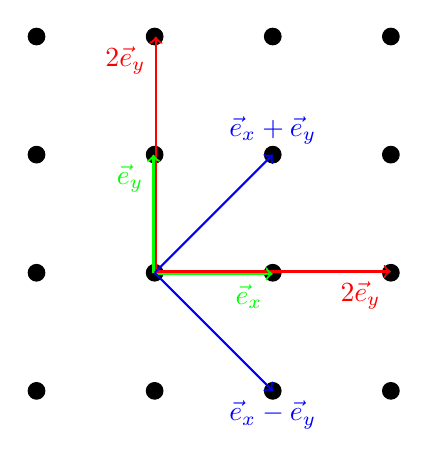
\begin{tikzpicture}[scale=1.5]
 \foreach \x in {1,...,4}
 \foreach \y in {1,...,4}
 \filldraw  (\x,\y) circle (2pt);
 \draw[->,red  ,thick] (2.01,2) -- (2.01,4) node[anchor=north east] {$2\vec e_y$};
 \draw[->,red  ,thick] (2,2.01) -- (4,2.01) node[anchor=north east] {$2\vec e_y$};
 \draw[->,green,thick] (1.99,2) -- (1.99,3) node[anchor=north east] {$\vec e_y$};
 \draw[->,green,thick] (2,1.99) -- (3,1.99) node[anchor=north east] {$\vec e_x$};
 \draw[->,blue ,thick] (2,2) -- (3,3) node[anchor= south] {$\vec e_x+ \vec e_y$};
 \draw[->,blue ,thick] (2,2) -- (3,1) node[anchor=north ] {$\vec e_x- \vec e_y$}; 
 \end{tikzpicture}
\end{center}
\caption{translation vectors $\vec T_d$ in a two dimensional square grid with first (green), second (blue) and third (red) neighbour interactions}
\label{2d_square}
\end{figure}

In an more elaborate approach we might add second and third neighbour hoppings. 
They can be treated in the same manner as nearest neighbours, simply by including the corresponding vectors $\vec T_d$ with their respective couplings.
The vectors up to third neighbour interactions are shown in figure \ref{2d_square}. 
We extend the single-particle Hamiltonian in real space to
\begin{IEEEeqnarray}{rCl}
 \hat{H}_0 &=& 
 - t \sum_{\langle i,j \rangle,\sigma} \left( c^{\dagger}_{i,\sigma}c_{j,\sigma} + c^{\dagger}_{j,\sigma}c_{i,\sigma} \right)
 - t^{\prime} \sum_{\langle \langle i,j \rangle \rangle ,\sigma} \left( c^{\dagger}_{i,\sigma}c_{j,\sigma} +c^{\dagger}_{j,\sigma}c_{i,\sigma} \right) \nonumber \\ &&
 - t^{\prime \prime} \sum_{\langle \langle \langle i,j \rangle \rangle \rangle ,\sigma} \left( c^{\dagger}_{i,\sigma}c_{j,\sigma}   + c^{\dagger}_{j,\sigma}c_{i,\sigma} \right)
 -\mu \sum_{i,\sigma} c^{\dagger}_{i,\sigma}c_{i;\sigma}
\end{IEEEeqnarray}
Double and triple brackets denote second- and third-neighbour pairs respectively and again, the sum counts each pair only once.
The resulting expression for the energy dispersion reads
\begin{equation}
 \varepsilon_{\vec k } = -2t \left(\cos k_x + \cos k_y \right) -4t^{\prime} \cos k_x \cos k_y  -2t^{\prime \prime} \left( \cos 2k_x + \cos 2k_y \right)
\end{equation}




The interaction term translates to
\begin{IEEEeqnarray}{rl}
 &\frac{U}{N^2} \sum_{\vec{k}\vec{l}\vec{m}\vec{n}} \sum_i \euler^{-\im (\vec{k}-\vec{l}+\vec{m}-\vec{n})\vec{R}_i } 
    c^{\dagger}_{\vec{k},\uparrow}c_{\vec{l},\uparrow} c^{\dagger}_{\vec{m},\downarrow}c_{\vec{n},\downarrow} \nonumber \\
    =& \frac{U}{N} \sum_{\vec{k}\vec{l}\vec{m}\vec{n}} \delta(\vec{k}-\vec{l}+\vec{m}-\vec{n} )
	c^{\dagger}_{\vec{k},\uparrow}c_{\vec{l},\uparrow} c^{\dagger}_{\vec{m},\downarrow}c_{\vec{n},\downarrow} \nonumber \\
    =& \frac{U}{N} \sum_{\vec{k}\vec{k}^{\prime}\vec{q}}
	c^{\dagger}_{\vec{k},\uparrow}c_{\vec{k}-\vec{q},\uparrow} c^{\dagger}_{\vec{k}^{\prime},\downarrow}c_{\vec{k}^{\prime}+\vec{q},\downarrow}
 \end{IEEEeqnarray}
where we choose a convenient parametrization for the sum over the momenta in the last line.
This term is non-diagonal, but it ensures momentum conversation at each vertex.

The total expression for the Hamiltonian in momentum space reads
 \begin{equation}
  \hat{H} = \sum_{\vec{k},\sigma} \left(\varepsilon_{\vec k} - \mu\right) c^{\dagger}_{\vec{k},\sigma}c_{\vec{k}\sigma} + \frac{U}{N} \sum_{\vec{k}\vec{k}^{\prime}\vec{q}}
	c^{\dagger}_{\vec{k},\uparrow}c_{\vec{k}-\vec{q},\uparrow} c^{\dagger}_{\vec{k}^{\prime},\downarrow}c_{\vec{k}^{\prime}+\vec{q},\downarrow}
 \end{equation} 

\section{Mean Field Equations}

\subsubsection{The Mean-Field Hamiltonian}

We treat the Hubbard model in a pertubative approach at the mean-field level.
The Hubbard term  $H_U$ acts as the pertubation.
As a two-particle operator it can be read as a product of two single particle opearators.
We can rewrite any product of two operators $\hat{A}$ and $\hat{B}$ as
\begin{IEEEeqnarray}{rCl}
 \hat{A}\cdot\hat{B} 
		    &=&	 \left(\hat A - \langle \hat A \rangle \right) \left( \hat B -\langle \hat B \rangle \right)
			 +\langle \hat A \rangle \hat B
			 +\langle \hat B \rangle \hat A
			 - \langle \hat A \rangle \langle \hat B \rangle
\end{IEEEeqnarray}
In the mean field approach we neglect the first term on the right hand side –the product of fluctuations around their expectation value– leaving us with
\begin{equation}
  \hat{A}\cdot\hat{B} 
		   \approx 
			 \langle \hat A \rangle \hat B
			 +\langle \hat B \rangle \hat A 
			 - \langle \hat A \rangle \langle \hat B \rangle
\end{equation}
% RPA has nothing to do with this I think…
%
We use this relation on the single particle oparators 
$c^{\dagger}_{\vec k,\uparrow}c_{\vec k - \vec q,\uparrow}$
and 
$c^{\dagger}_{\vec k,\downarrow}c_{\vec k + \vec q,\downarrow}$
in the Hubbard term of the Hamiltonian. 
Furthermore, we drop the constant term corresponding to $\langle \hat A \rangle \langle \hat B \rangle$, since a constant in the Hamiltonian will not have any
influence on the dynamic of the system. 
The mean-field approxiamtion of the Hubbard term reads
\begin{equation}
 H_U \stackrel{\mathrm{mf}}{\approx}  \frac{U}{N}
 \sum_{\vec{q}} \sum_{\sigma} 
 \left( \sum_{\vec{p}^{\prime}} \langle c^{\dagger}_{\vec{p}^{\prime},-\sigma} c_{\vec{p}^{\prime}+\vec{q},-\sigma} \rangle \right)
	\sum_{\vec p}  c^{\dagger}_{\vec{p},\sigma} c_{\vec{p}-\vec{q},\sigma}. \label{Hubbard_mean_field}
\end{equation}
The expectation value for the one particle operator is different from zero for only two values of $\vec q$.
First, for $\vec q = 0$ the expression yields the spin dependent filling factor, i.e. the number of particles with spin $\sigma$ in relation to the total number of sites $N$.
\begin{equation}
 n_{\sigma} = \frac1N \sum_{\vec k} \langle c^{\dagger}_{\vec k, \sigma} c_{\vec k, \sigma} \rangle.
\end{equation}
Due to the Pauli principle we can have only one particle with a certain spin at each site. This value is therefore restricted to the range $[0,1]$.
The total number density is simply the sum of both spin dependent number densites, $n=n_{\uparrow}+n_{\downarrow}$ 
and ranges from 0 for the empty case to 2, corresponding to a situation where each sites is occupied by two particles with opposite spin.

%
%
% meaning of mean-field
%
% symmetry bracking, antiferromagnetic ground state
%
%propagators: diagonal, offdiagonal
%
% validity range of the above assumptions: symmetrie, metal insulator transition; limits and corrections
%
%RPA
%
%
The second contribution comes from $\vec q = (\frac12, \frac12)$.
This vector acts as a nesting vector for the Fermi surface of the band structure. 
A square lattice with only nearest-neighbour interactions can be divided into two sublattices. 
Hoppings occur only from one sublattice to the other and as a result we get a perfectly nested energy dispersion,
that is
$\varepsilon_{\vec k} = -\varepsilon_{\vec k + \vec Q}$ with the nesting vector $\vec Q = (\frac12,\frac12)$ in units of $2\pi$.
The Fermi surface in this case is therefore a perfect square. 
Introducing higher order hopping terms deforms it, but nesting with $\vec Q$ holds on a approximate level for small $t^{\prime}$ and $t^{\prime \prime}$.
The Fermi surfaces with nesting vector $\vec Q$ for two different sets of parameters are shown in \ref{fig:energie_dispersion}.
%
%
\begin{figure} \centering
\begin{subfigure}{0.49\linewidth} \centering
 \includegraphics[width=\textwidth]{../bandstructure_t.pdf}
 \caption{$ t^{\prime}=t^{\prime \prime} =0$ }
 \label{fig:dispt}
\end{subfigure}
\begin{subfigure}{0.49\linewidth}
  \includegraphics[width=\textwidth]{../bandstructure_ttt.pdf}
  \caption{ $t^{\prime}= 0.2326t$, $t^{\prime \prime} = 0.1163t$}
  \label{fig:dispttt}
\end{subfigure}
\caption{single particle energy dispersion in units of t with nesting vector $\vec Q$. }
\label{fig:energie_dispersion}
\end{figure}
%
%$\vec Q$ is the basis vector for antiferromagnetic ordering. 
%This is observed in these materials \todo{how general, which ones} and expected % for what reason?
Nesting with $\vec Q = (\frac 12, \frac12)$ leads to a symmetrie broken ground state with an antiferromagnetic moment. 
\todo{why do we expect SB? How does this arise from a nested Fermi surface?}


reference for AF GS:
\cite{PhysRevLett.62.591}


The expectation value of the staggered magnetization, given by
\begin{IEEEeqnarray}{lCl}
 m_{s} &=& m_{s, \uparrow} - m_{s, \downarrow}, \\
 m_{s, \sigma} &=& \frac1N \sum_{\vec k} \langle c^{\dagger}_{\vec k , \sigma} c_{\vec k + \vec Q, \sigma} \rangle,
\end{IEEEeqnarray}
is therefore non-zero. 

In terms of the above defined parameters equation \ref{Hubbard_mean_field} simplifies finally to
\begin{equation}
 \hat H = \sum_{\vec k, \sigma} \left( \varepsilon_{\vec k } - \mu + U n_{-\sigma} \right) c^{\dagger}_{\vec k, \sigma} c_{\vec k ,\sigma}
	  + U m_{s,-\sigma} \sum_{\vec k, \sigma} c^{\dagger}_{\vec k + \vec Q, \sigma} c_{\vec k, \sigma}.
\end{equation}
%
%\begin{equation}
% H_U \approx \sum_{\sigma} \left( U n_{-\sigma} \sum_{\vec{p}} c^{\dagger}_{\vec{p}, \sigma} c_{\vec p, \sigma} 
%	      + \frac{ U m_{s,-\sigma}}2
%			      \sum_{\vec p} \left(  c^{\dagger}_{\vec{p}+\vec Q, \sigma} c_{\vec p, \sigma} 
%	                                          + c^{\dagger}_{\vec{p}       , \sigma} c_{\vec p+ \vec Q, \sigma} \right) \right)
%\end{equation}
%
%\begin{IEEEeqnarray}{rCl}
% H_{\mathrm{mf}} &=
%		\sum_{\vec{p},\sigma} &
%				      \left( \varepsilon_{\vec k} - \mu + U n_{-\sigma} \right) 
%					  c^{\dagger}_{\vec{p},\sigma} c_{\vec{p},\sigma}
%				      +\frac{U}2  m_{s,-\sigma}	 
%					  \left( c^{\dagger}_{\vec{p}+\vec{Q},\sigma} c_{\vec{p},\sigma} +\mathrm{h.c.} %c^{\dagger}_{\vec{p},\sigma} c_{\vec{p}+\vec{Q},\sigma} 
%					  \right)					 
%\end{IEEEeqnarray}
%
We are left with a Hamilton operator consisting only of single particle operators. 
That shows the idea of the mean-field approach, describing non-interacting particles that are exposed to an averaged field.
This averaged field is the result off these particles in the system. It's value will therefore be influenced by the particles itself.
As a result we have to solve the equations for the fields self-consistently, which will be done in the next section. 
The first term in the above mean-field Hamiltonian represents the mean repulsion due to the equal charge of the electrons.
It is proportional to the number density of particles with opposite spin due to the on-site interaction, that is only possible for particles with opposite spin.
The second term corresponds to the coupling to a staggered magnetic field, that is a magnetic field with an alternating orientation on each site. 
The field strength is proportional to the magentization of the ground state and given by $Um_s$.

\subsubsection{Mean-Field Propagators}

The mean-field Hamiltonian gives rise to two different propagators.
First we get the diagonal contribution, second an off-diagonal one from the staggered component. 
The propagators are defined by
\begin{IEEEeqnarray}{rCl}
 G_{\vec k}(\tau) &=& -\langle \mathcal{T}_{\tau} c_{\vec k         ,\sigma}(\tau)  c^{\dagger}_{\vec k ,\sigma}(0) \rangle \\
 F_{\vec k}(\tau) &=& -\langle \mathcal{T}_{\tau} c_{\vec k +\vec{Q},\sigma}(\tau)  c^{\dagger}_{\vec k ,\sigma}(0) \rangle \\ \label{Def_Propagator}
\end{IEEEeqnarray}
with the imaginary time ordering operator $\mathcal{T}_{\tau}$, acting on a pair of fermion operators according to
\begin{IEEEeqnarray}{rCl}
 \mathcal{T}_{\tau} \hat{A}(\tau_1) \hat{B}(\tau_2) &=&
 -\Theta(\tau_1-\tau_2)\hat{A}(\tau_1) \hat{B}(\tau_2) + \Theta(\tau_2-\tau_1)\hat{B}(\tau_2) \hat{A}(\tau_1) \nonumber \\
 &=& \left\{ \begin{array}{r@{\text{ for }}l} -\hat{A}(\tau_1) \hat{B}(\tau_2) & \tau_1 \ge \tau_2 \\ \hat{B}(\tau_2) \hat{A}(\tau_1) & \tau_1 < \tau_2 \end{array} \right.
\end{IEEEeqnarray}
For the behaviour at $\tau=0$ as shown in the last line, we need the convetion of $\Theta(0)=\frac12$.
From this definition follows that $n_\sigma$ and $m_{s,\sigma}$ can be expressed in terms of propagators, namely through
\begin{IEEEeqnarray}{lCl}
 n_{\sigma} &=& \frac1N \sum_{\vec k} \left( 1-G_{\vec k, -\sigma}(0) \right) \label{n_DEF}\\
 m_{s,\sigma} &=& -\frac1N \sum_{\vec k} F_{\vec k, -\sigma}(0)		\label{m_DEF}
\end{IEEEeqnarray}


From the definition of the propagtors in \ref{Def_Propagator} and the equation of motion for operators, 
$\frac{\dint}{\dint \tau} \hat{A} = [H,\hat{A}] + \frac{\partial}{\partial_{\tau}} \hat{A}$,
we get the differential equation
\begin{IEEEeqnarray}{rCl}
 \partial_{\tau} G_{\vec k ,\sigma}(\tau) 
 &=&
 \delta(\tau) \langle c_{\vec k ,\sigma}(\tau) c^{\dagger}_{\vec k ,\sigma}(0) + c^{\dagger}_{\vec k ,\sigma}(0) c_{\vec k ,\sigma}(\tau) \rangle \nonumber \\&&
 + \Theta(\tau) \langle [\hat H , c_{\vec k ,\sigma}(\tau)] c^{\dagger}_{ \vec k ,\sigma}(0) \rangle		\nonumber \\ &&
 -  \Theta(-\tau) \langle c^{\dagger}_{ \vec k ,\sigma}(0) [\hat H , c_{\vec k ,\sigma}(\tau)]  \rangle \label{EOM_G}
\end{IEEEeqnarray}
Here we used $\partial_{\tau} \Theta(\tau) = \delta(\tau)$.
The commutators can be evaluated using the identity $[AB,C] = A\{B,C\} - \{A,C\}B$ and the anticommutation rules for the creation and annihilation operators.
\todo{give fermion commutation rules somewhere earlier}
This leaves us with
\begin{equation}
 [H,c_{\vec k ,\sigma}(\tau)]=-\left(\varepsilon_{\vec k}-\mu + Un_{-\sigma} \right) c_{\vec k ,\sigma}(\tau) - Um_{s,-\sigma} c_{\vec k +\vec{Q},\sigma}(\tau)
\end{equation}
Putting this back in \ref{EOM_G} together with the definitions for $G$ and $F$, we get
\begin{IEEEeqnarray}{rCl}
  \partial_{\tau} G_{\vec k ,\sigma}(\tau) 
&=&
\delta(\tau)\langle \{c_{\vec k ,\sigma}(\tau),c^{\dagger}_{\vec k ,\sigma}(0)\} \rangle
- \left( \varepsilon_{\vec k }-\mu+ Un_{-\sigma} \right) G_{\vec k ,\sigma}(\tau)  \nonumber \\ &&
 -Um_{s,-\sigma} F_{\vec k ,\sigma}(\tau) \label{EOM_G_II}
\end{IEEEeqnarray}
In a next step we take the Fourier transform of this equation. 
The Fourier transformed propagator is related to the propagator in imaginary time through
\begin{IEEEeqnarray}{rCl}
 G_{\vec k ,\sigma}(\tau) &=& \frac{1}{\beta} \sum_n \euler^{-\im \omega_n \tau} G_{\vec k ,\sigma}(\im \omega_n) \\
 G_{\vec k ,\sigma}(\im \omega_n) &=& \int_0^{\beta} \! \!\dint  \tau \: \euler^{\im \omega_n \tau} G_{\vec k ,\sigma}(\tau)
\end{IEEEeqnarray}
The so called Matsubara frequencies $\omega_n$ are given by $\omega_n = \frac{\pi}{\beta}(2n+1), \; n \! \in \! \mathbb{Z}$.
This ensures the anti-periodicity of fermionic Greensfunctions, $G(\tau+\beta) = -G(\tau)$.
Transforming equation \ref{EOM_G_II} to momentum space we get
\begin{IEEEeqnarray}{rCl}
 \left( \im \omega_n -\varepsilon_{\vec k } +\mu - Un_{-\sigma} \right) G_{\vec k ,\sigma}(\im \omega_n) = 1 +Um_{s,-\sigma} F_{\vec k ,\sigma}(\im \omega_n)
\end{IEEEeqnarray}
In the same way, starting from $\frac{\dint}{\dint \tau} F_{\vec k ,\sigma}(\tau)$ we get for the off-diagonal propagator
\begin{IEEEeqnarray}{rCl}
 \left( \im \omega_n -\varepsilon_{\vec k +\vec{Q}} +\mu - Un_{-\sigma} \right) F_{\vec k ,\sigma}(\im \omega_n) = Um_{s,-\sigma} G_{\vec k ,\sigma}(\im \omega_n)
\end{IEEEeqnarray}
There is no constant term, since the anticommutator in \ref{EOM_G_II} is zero for off-diagonal momenta. 
Putting the last two equations together we get the expressions for the propagators
\begin{IEEEeqnarray}{rCl}
 G_{\vec k ,\sigma}(\im \omega_n) &=& \frac{ ( \im \omega_n - \varepsilon_{\vec k +\vec{Q}} + \mu -Un_{-\sigma} )}
			      { ( \im \omega_n - \varepsilon_{\vec k +\vec{Q}} + \mu -Un_{-\sigma} )
			        ( \im \omega_n - \varepsilon_{\vec k }         + \mu -Un_{-\sigma} )
			      - U^2m_{s,-\sigma}^2 } \nonumber \\
 F_{\vec k ,\sigma}(\im \omega_n) &=& \frac{ Um_{s,-\sigma}}
			    { ( \im \omega_n - \varepsilon_{\vec k +\vec{Q}} + \mu -Un_{-\sigma} )
			      ( \im \omega_n - \varepsilon_{\vec k }         + \mu -Un_{-\sigma} )
			      - U^2m_{s,-\sigma}^2 }			      
\end{IEEEeqnarray}
We can rewrite this in a more appealing way by factorizing the denominator of both propagators. 
The poles are located at
\begin{equation}
 E_{\vec k ,\sigma}^{\pm}
 =
 \frac{\varepsilon_{\vec k }+\varepsilon_{\vec k +\vec{Q}}}2 -\mu + Un_{-\sigma}  \pm \sqrt{ \left(\frac{\varepsilon_{\vec k }-\varepsilon_{\vec k +\vec{Q}}}2\right)^2 + U^2m_{s,-\sigma}^2 }
\end{equation}
Note that $E_{\vec k ,\sigma}^{\pm}=E_{\vec k +\vec{Q},\sigma}^{\pm}$, since $\varepsilon_{\vec k +2\vec{Q}}=\varepsilon_{\vec k }$.
Using these expressions the propagators can be expressed as
\begin{IEEEeqnarray}{rCl}
 G_{\vec k ,\sigma}(\im \omega_n) &=& \frac{ \im \omega_n - \varepsilon_{\vec k +\vec{Q}} +\mu -Un_{-\sigma} }
					    { (\im \omega_n - E_{\vec k ,\sigma}^+) (\im \omega_n - E_{\vec k ,\sigma}^-) }
\\
 F_{\vec k ,\sigma}(\im \omega_n) &=& \frac{ Um_{s,-\sigma} }
					    { (\im \omega_n - E_{\vec k ,\sigma}^+) (\im \omega_n - E_{\vec k ,\sigma}^-)}
\end{IEEEeqnarray}
We note that $F_{\vec k,\sigma}$ is invariant under a translation $\vec k \rightarrow \vec k +\vec Q$, 
while $G_{\vec k,\sigma}$ changes depending on the dispersion $\varepsilon_{\vec k}$.


%\begin{IEEEeqnarray}{rCl}
%  G_{\vec{p},\sigma}(\im \omega_n) &=& \frac{ u_{\vec{p}        ,\sigma }}{ (\im \omega_n - E_{\vec{p},\sigma}^+) }
%			+ \frac{ u_{\vec{p}+\vec{Q},\sigma }}{ (\im \omega_n - E_{\vec{p},\sigma}^-) } \\
%  F_{\vec{p},\sigma}(\im \omega_n) &=& \frac{ \tilde{u}_{\vec{p},\sigma }}{ (\im \omega_n - E_{\vec{p},\sigma}^+) }
%			- \frac{ \tilde{u}_{\vec{p},\sigma }}{ (\im \omega_n - E_{\vec{p},\sigma}^-) }
%\end{IEEEeqnarray}
%where $u$ and $\tilde{u}$ are given by
% \begin{IEEEeqnarray}{rCl}
% u_{\vec{p},\sigma} &=& \frac{E_{\vec{p},\sigma}^+ - \varepsilon_{\vec{p}+\vec{Q}} +\mu -Un_{-\sigma} }{E_{\vec{p},\sigma}^+ -E_{\vec{p},\sigma}^-} \\
% \tilde{u}_{\vec{p},\sigma} &=& \frac{Um_{s,-\sigma}}{E_{\vec{p},\sigma}^+ -E_{\vec{p},\sigma}^-}.
% \end{IEEEeqnarray}
% \todo{connection to diagrammatic approach, resolve $1-n_{-\sigma} \stackrel{?}{=} n_{-\sigma}$ issue.} 
% \todo{ How to draw nice diagrams in \LaTeX?}

There is an alternative approach from a diagrammatic point of view, that gives the same differential equation for the propagators.
Following the notation of \ref{PhysRevB.65.132404}, 
we denote the bare propagator $G^0_{\vec k,\sigma}$ by a single line, the mean-field propagators by double lines and the interaction by a dashed line.
The off-diagonal propagator $F_{\vec k ,\sigma}$ is marked with an doubled arrow head.
The diagrams for a self-consistent mean-field approximation are shown in figure \ref{Diagr_Props}. 
%
By including only single loops we neglect again the possiblity of quantum fluctuations, i.e. there are no interactions with virtual states.
Note that the particles on each site of the interaction have different spins and there is no spin transfer. 
The straight arrows have therefore all the same spin, while all particles in the loops have the opposite spin.
We reflect the sum up to infinite such interactions by using the mean-field propagator after the interaction. 
%
Self-consistency is achieved by using the mean-field propagators in the loops.
This reflects the fact, that $m_{s,\sigma}$ and $n_{\sigma}$ itself depend on the sum over the respective mean-field propagator.
As a result we have to solve the equations for $m_{s,\sigma}$ and $n_{\sigma}$ iteratively. % CHECK IF THIS SENTENCE APPEARS LATER AGAIN.
%
Inserting the bare propagator ${G^0_{\vec k,\sigma}(\im \omega_n)}=(\im \omega_n +\varepsilon_{\vec k} - \mu)^{-1}$ of the non interacting system
as well as equations \ref{n_DEF} and \ref{m_DEF}
reproduces the above expressions for $G_{\vec k, \sigma}$ and $F_{\vec k ,\sigma}$.


\begin{fmffile}{prop}

\fmfcmd{%
style_def dbl_plain_dbl_arrow expr p =
draw_double p;
shrink(1.5);
cfill (harrow (p, 0.8));
cfill (harrow (p, 0.7));
endshrink;
enddef;}

\begin{figure}
 \centering
\begin{IEEEeqnarray}{rCl}
 \parbox{20mm}{
	      \begin{fmfgraph}(20mm,30mm)
		\fmfleft{i1}
		\fmfright{o1}
		\fmf{dbl_plain_arrow}{i1,o1}
	      \end{fmfgraph}
	      }
&=& \parbox{15mm}{\begin{fmfgraph}(15mm,30mm) \fmfleft{i} \fmfright{o} \fmf{plain_arrow}{i,o} \end{fmfgraph}} 
   + \parbox{25mm}{\begin{fmfgraph}(25mm,30mm) \fmfleft{i1} \fmfright{o1} \fmf{plain_arrow}{i1,v1} \fmf{dbl_plain_dbl_arrow}{v1,o1}
					   \fmf{dashes,tension=0}{v2,v1} 	 \fmfforce{0.5w,.8h}{v2}     \fmf{dbl_plain_dbl_arrow}{v2,v2}
                \end{fmfgraph} }
	+    \parbox{25mm}{\begin{fmfgraph}(25mm,30mm) \fmfleft{i1} \fmfright{o1} \fmf{plain_arrow}{i1,v1} \fmf{dbl_plain_arrow}{v1,o1}
					   \fmf{dashes,tension=0}{v2,v1} 	 \fmfforce{0.5w,.8h}{v2}     \fmf{dbl_plain_arrow}{v2,v2} \end{fmfgraph} }
\end{IEEEeqnarray}
 \begin{IEEEeqnarray}{rCl}
 \parbox{20mm}{
	      \begin{fmfgraph}(20mm,30mm)
		\fmfleft{i1}
		\fmfright{o1}
		\fmf{dbl_plain_dbl_arrow}{i1,o1}
	      \end{fmfgraph}
	      }
&=& \parbox{25mm}{\begin{fmfgraph}(25mm,30mm) \fmfleft{i1} \fmfright{o1} \fmf{dbl_plain_dbl_arrow}{i1,v1} \fmf{plain_arrow}{v1,o1}
					   \fmf{dashes,tension=0}{v2,v1} 	 \fmfforce{0.5w,.8h}{v2}     \fmf{dbl_plain_arrow}{v2,v2}
                \end{fmfgraph} }
	+    \parbox{25mm}{\begin{fmfgraph}(25mm,30mm) \fmfleft{i1} \fmfright{o1} \fmf{plain_arrow}{i1,v1} \fmf{dbl_plain_arrow}{v1,o1}
					   \fmf{dashes,tension=0}{v2,v1} 	 \fmfforce{0.5w,.8h}{v2}     \fmf{dbl_plain_dbl_arrow}{v2,v2} \end{fmfgraph} }
\end{IEEEeqnarray} 
\label{Diagr_Props}
\caption{Self consistent mean-field equations for $G_{\vec k, \sigma}$ and $F_{\vec k, \sigma}$.}
\end{figure} 
 


\subsubsection{Validity of Mean-Field Description}
% This should maybe be the first point in the mean-field section
%In order to treat the Hubbard model in the mean-field approach we rely on assumptions. that limit this approach to a certain set of parameters.
% Antiferromagnetic groundstate – low T
% low fluctuations
% Mott insulator
% effect of quantum fluctuations





\section{Observables}

\subsection{Response Functions}

\subsection{X-Ray and Neutron Scattering Experiments}

\subsection{Calculating the Dynamic Magnetic Susceptibility}

In experiments revealing the properties of those materials, one usually measures response functions. 
They describe the reaction of the material to a external parameter like a electromagnetic field.
For sufficient weak fields the response will be linear.
A linear response function can be expressed in term of four-point Greens functions.

In X-Ray or neutron scattering experiments the obeservable quantity is the differential scattering cross section, which is related to the dynamic magnetic susceptibility via
\begin{equation}
\frac{\dint^2 \sigma}{\dint \Omega \dint \omega} = -2\Im \left(\chi(\omega,\vec q)\right)
\end{equation}
\todo{derivation from Fermis Golden Rule in Appendix}




The dynamical spin susceptibility can be expressed as
\begin{equation}
 \chi_{J}^{ab} = \delta_{ab} \langle \mathbf{J}(\vec q,\tau)\cdot \mathbf{J}(-\vec q,) \rangle
\end{equation}
with the components 
\begin{equation}
\mathbf{ J}^{a}(\vec q) = \sum_{\vec k} \sum_{\alpha,\beta} c^{\dagger}_{\vec k ,\alpha} \left(\sigma^a \right)_{\alpha\beta} c_{\vec k+\vec q,\beta}
\end{equation}



\begin{equation}
 \chi_J(\vec q,\omega)  = \chi_J^{+-}(\vec q,\omega) + \chi_J^{-+}(\vec q,\omega) + \chi_J^{zz}(\vec q,\omega)
\end{equation}




%The components of the magnetic susceptibility are defined by
%\begin{equation}
% \chi^{ab}(\tau - \tau^{\prime}) = \sum_{\vec{p}} \left( \sum_{\alpha, \beta} c^{\dagger}_{\vec k, \alpha }(\tau) \left(\sigma^{a}\right)_{\alpha \beta} c_{\vec k , \beta}(\tau)  \right)
%			    \cdot \left(  \sum_{\gamma, \delta} c^{\dagger}_{\vec k, \gamma }(\tau^{\prime}) \left(\sigma^{b}\right)_{\gamma \delta} c_{\vec k , \delta}(\tau^{\prime}) \right)  
%\end{equation}


Expressing $\chi_J^{+-}$ and $\chi_J^{-+}$ in creation and destruction operators gives then
\begin{IEEEeqnarray}{rCl}
 \chi^{+-}(\vec q,\omega) &=& \int_0^{\beta} \!\!\dint \tau \euler^{\im \omega \tau} \langle \mathcal{T}_{\tau} S^+(\vec q,\tau) S^-(-\vec q,0) \rangle \nonumber \\
			  &=&  \sum_{\vec k \vec k^{\prime}} \langle c^{\dagger}_{\vec k,\downarrow}(\tau) c_{\vec k+\vec q, \uparrow}(\tau) 
								    c^{\dagger}_{\vec k^{\prime}+\vec q,\downarrow}(0) c_{\vec k^{\prime},\uparrow}(0) \rangle
\end{IEEEeqnarray}

\begin{IEEEeqnarray}{rCl}
 \chi^{+-}(\vec q,\omega) &=& \int_0^{\beta} \!\!\dint \tau \euler^{\im \omega \tau} \langle \mathcal{T}_{\tau} S^+(\vec q,\tau) S^-(-\vec q,0) \rangle \nonumber \\
			  &=&  \sum_{\vec k \vec{p}^{\prime}} \langle c^{\dagger}_{\vec k,\downarrow}(\tau) c_{\vec k+\vec q, \uparrow}(\tau) 
								    c^{\dagger}_{\vec k^{\prime}+\vec q,\downarrow}(0) c_{\vec k^{\prime},\uparrow}(0) \rangle
\end{IEEEeqnarray}

can be expressed in terms of the above Greens functions.
We expand the expression in terms of ladder diagrams.
The first order bubble diagrams are shown in figure \ref{bubbles}.


\begin{figure}
\begin{tabular}{ccc}
 \begin{fmfgraph*}(120,45)
  \fmfleft{i1} \fmfright{o1} \fmf{dots_arrow,tension=2,label=$\vec q$}{i1,v1} \fmf{dbl_plain_arrow,left=.35}{v1,v2,v4} 
  \fmf{dbl_plain_arrow,left=.35}{v4,v3,v1} \fmf{dots_arrow,tension=2,label=$\vec q$}{v4,o1}
  \fmfforce{.5w,h}{v2} \fmfforce{.5w,0}{v3} \fmf{dashes,tension=0}{v2,v3}
 \end{fmfgraph*}
 &
 \begin{fmfgraph*}(120,45)
  \fmfleft{i1} \fmfright{o1} \fmf{dots_arrow,tension=2,label=$\vec q$}{i1,v1} \fmf{dbl_plain_arrow,left=.35}{v1,v2,v4} 
  \fmf{dbl_plain_arrow,left=.35}{v4,v3,v1} \fmf{dots_arrow,tension=2,label=$\vec q$}{v4,o1}
  \fmfforce{.5w,h}{v2} \fmfforce{.5w,0}{v3} \fmf{dashes,tension=0}{v2,v3}
 \end{fmfgraph*}
 &
 \begin{fmfgraph*}(120,45)
  \fmfleft{i1} \fmfright{o1} \fmf{dots_arrow,tension=2,label=$\vec q$}{i1,v1} \fmf{dbl_plain_arrow,left=.35}{v1,v2,v4} 
  \fmf{dbl_plain_arrow,left=.35}{v4,v3,v1} \fmf{dots_arrow,tension=2,label=$\vec q$}{v4,o1}
  \fmfforce{.5w,h}{v2} \fmfforce{.5w,0}{v3} \fmf{dashes,tension=0}{v2,v3}
 \end{fmfgraph*}
 \\
 \begin{fmfgraph*}(120,45)
  \fmfleft{i1} \fmfright{o1} \fmf{dots_arrow,tension=2,label=$\vec q$}{i1,v1} \fmf{dbl_plain_dbl_arrow,left=.35}{v1,v2,v4} 
  \fmf{dbl_plain_dbl_arrow,left=.35}{v4,v3,v1} \fmf{dots_arrow,tension=2,label=$\vec q$}{v4,o1}
  \fmfforce{.5w,h}{v2} \fmfforce{.5w,0}{v3} \fmf{dashes,tension=0}{v2,v3}
 \end{fmfgraph*}
 &
 \begin{fmfgraph*}(120,45)
  \fmfleft{i1} \fmfright{o1} \fmf{dots_arrow,tension=2,label=$\vec q$}{i1,v1} \fmf{dbl_plain_arrow,left=.35}{v1,v2,v4} 
  \fmf{dbl_plain_arrow,left=.35}{v4,v3,v1} \fmf{dots_arrow,tension=2,label=$\vec q$}{v4,o1}
  \fmfforce{.5w,h}{v2} \fmfforce{.5w,0}{v3} \fmf{dashes,tension=0}{v2,v3}
 \end{fmfgraph*}
 &
 \begin{fmfgraph*}(120,45)
  \fmfleft{i1} \fmfright{o1} \fmf{dots_arrow,tension=2,label=$\vec q$}{i1,v1} \fmf{dbl_plain_arrow,left=.35}{v1,v2} \fmf{dbl_plain_dbl_arrow,left=.35}{v2,v4} 
  \fmf{dbl_plain_arrow,left=.35}{v4,v3} \fmf{dbl_plain_dbl_arrow,left=.35}{v3,v1} \fmf{dots_arrow,tension=2,label=$\vec q$}{v4,o1}
  \fmfforce{.5w,h}{v2} \fmfforce{.5w,0}{v3} \fmf{dashes,tension=0}{v2,v3}
 \end{fmfgraph*}
 \\
 \begin{fmfgraph*}(120,45)
  \fmfleft{i1} \fmfright{o1} \fmf{dots_arrow,tension=2,label=$\vec q$}{i1,v1} \fmf{dbl_plain_arrow,left=.35}{v1,v2,v4} 
  \fmf{dbl_plain_dbl_arrow,left=.35}{v4,v3,v1} \fmf{dots_arrow,tension=2,label=$\vec q$}{v4,o1}
  \fmfforce{.5w,h}{v2} \fmfforce{.5w,0}{v3} \fmf{dashes,tension=0}{v2,v3}
 \end{fmfgraph*}
 &
 \begin{fmfgraph*}(120,45)
  \fmfleft{i1} \fmfright{o1} \fmf{dots_arrow,tension=2,label=$\vec q$}{i1,v1} \fmf{dbl_plain_dbl_arrow,left=.35}{v1,v2,v4} 
  \fmf{dbl_plain_arrow,left=.35}{v4,v3,v1} \fmf{dots_arrow,tension=2,label=$\vec q$}{v4,o1}
  \fmfforce{.5w,h}{v2} \fmfforce{.5w,0}{v3} \fmf{dashes,tension=0}{v2,v3}
 \end{fmfgraph*} &
 \end{tabular}
 \label{bubbles}
 \caption{first order diagrams contributing to $\chi^{+-}(\vec q, \im \omega_n)$.}
\end{figure}


Taking only ladder and bubble diagrams into account is known as the random phase approximation (RPA) which once again neglects quantum fluctuations. 
The contribution from these fluctuations vanish in the large $N$ limit.
\todo{non-crossing approximation}
The building blocks of each step in the ladder consists of a product of two propagators. 
The building blocks for the ladder diagrams are listed in table \ref{blocks}.


\begin{table}
\centering
\begin{tabular}{|c|V|c|}
\hline
 $\lambda$ &  
 \begin{fmfgraph}(60,35)
  \fmfleft{i1,i2} \fmfright{o1,o2}  \fmf{dashes,tension=0}{i1,i2} \fmf{phantom}{i1,o1} \fmf{phantom}{i2,o2}
 \end{fmfgraph}
 & $\frac UN$  \\[.8cm]
 %
 $\lambda x$ & 
\begin{fmfgraph*}(60,35)
  \fmfleft{i1,i2} \fmfright{o1,o2}  \fmf{dashes,tension=0}{i1,i2} \fmf{dbl_plain_arrow}{o1,i1} \fmf{dbl_plain_arrow}{i2,o2}
  \fmfv{l=$\uparrow$,l.a=25,l.d=1}{o1}
  \fmfv{l=$\downarrow$,l.a=-25,l.d=1}{o2}
 \end{fmfgraph*}
 & $\frac UN\sum_{\vec k,n^{\prime}} G_{\vec k, \downarrow}(\im \omega_{n^{\prime}}) G_{\vec k +\vec q,\uparrow }(\im \omega_{n^{\prime}} + \im \omega_n)$ \\[.8cm]
 %
 $\lambda y$ &
\begin{fmfgraph*}(60,35)
  \fmfleft{i1,i2} \fmfright{o1,o2}  \fmf{dashes,tension=0}{i1,i2} \fmf{dbl_plain_dbl_arrow}{o1,i1} \fmf{dbl_plain_dbl_arrow}{i2,o2}
  \fmfv{l=$\uparrow$,l.a=25,l.d=1}{o1}
  \fmfv{l=$\downarrow$,l.a=-25,l.d=1}{o2}
 \end{fmfgraph*} 
 & $\frac UN\sum_{\vec k,n^{\prime}} F_{\vec k, \downarrow}(\im \omega_{n^{\prime}}) F_{\vec k +\vec q,\uparrow }(\im \omega_{n^{\prime}} + \im \omega_n)$ \\[.8cm]
 %
 $\lambda z_1$ &
 \begin{fmfgraph*}(60,35)
  \fmfleft{i1,i2} \fmfright{o1,o2}  \fmf{dashes,tension=0}{i1,i2} \fmf{dbl_plain_dbl_arrow}{o1,i1} \fmf{dbl_plain_arrow}{i2,o2}
    \fmfv{l=$\uparrow$,l.a=25,l.d=1}{o1}
  \fmfv{l=$\downarrow$,l.a=-25,l.d=1}{o2}
 \end{fmfgraph*}
 &  $\frac UN\sum_{\vec k,n^{\prime}} G_{\vec k, \downarrow}(\im \omega_{n^{\prime}}) F_{\vec k +\vec q,\uparrow }(\im \omega_{n^{\prime}} + \im \omega_n)$ \\[.8cm]
 %
 $\lambda z_2$ &
 \begin{fmfgraph*}(60,35)
  \fmfleft{i1,i2} \fmfright{o1,o2}  \fmf{dashes,tension=0}{i1,i2} \fmf{dbl_plain_arrow}{o1,i1} \fmf{dbl_plain_dbl_arrow}{i2,o2}
   \fmfv{l=$\uparrow$,l.a=25,l.d=1}{o1}
  \fmfv{l=$\downarrow$,l.a=-25,l.d=1}{o2}
 \end{fmfgraph*}
 &  $\frac UN\sum_{\vec k,n^{\prime}} F_{\vec k, \downarrow}(\im \omega_{n^{\prime}}) G_{\vec k +\vec q,\uparrow }(\im \omega_{n^{\prime}} + \im \omega_n)$ \\
 \hline
\end{tabular}
\label{blocks}
\caption{building blocks of ladder diagrams for $\chi^{+-}(\vec q, \im \omega_n)$}
\end{table}

Momentum conversation at each vertex limits the sum over momenta in each block to $\vec k^{\prime} = \vec k + \vec q$ or $\vec k^{\prime} = \vec k + \vec q + \vec Q$
The second possibility is due to the off-diagonal propagator $F_{\vec k,\sigma}$, that adds $\vec Q$ to the momentum. 
Each block consists of a sum over momenta, we can therefore shift the momentum in the product of propagators without changing the value of the sum.
As mentioned above, only $G_{\vec k,\sigma}$ changes under a shift of $\vec Q$, $F_{\vec k,\sigma}$ however is invariant under such a transformation.
Therefore only $x$ will change it's value for $\vec q \rightarrow \vec q + \vec Q$, in all other situations the sum is unchanged, 
as the transformation can be absorbed in $F_{\vec k,\sigma}$,
We will write $\bar x$ to denote the expression for $x$ with $\vec k - \vec k^{\prime} = \vec q + \vec Q$. 

The infinite sum of bubble diagrams represents a geometric series and has an analytical expression.
In order to deal with the right momenta between upper and lower propagator we rewrite it as a $ 2 \times 2$ matrix equation and pick the value that 
corresponds to having $\vec q$ as the external momentum on both sides of the diagram.
The upper component in this matrix equation corresponds to $\vec k - \vec k^{\prime} = \vec q$, 
while the lower one corresponds to $\vec k -\vec k^{\prime} = \vec q + \vec Q$.
The full equation reads then
\begin{equation}
 \chi_{\mathrm{RPA}}^{+-}(\vec q,\im \omega_n) = 
 \left( \begin{array}{cc} x+y & z_1+z_2 \end{array} \right) \cdot \sum_{m=0}^{\infty} (-\lambda M)^m \cdot \left( \begin{array}{c} -1 \\  \: 0 \end{array} \right)
\end{equation}
with the matrix $M$ combining all the possibilities for one new step in the ladder for each order $m$,
\begin{equation}
M =  \left( \begin{array}{cc} x+y & z_1+z_2 \\
			       z_1+ z_2 & \bar x +  y  \end{array} \right)
\end{equation}
At the end of a ladder diagram however we have to fullfill $\vec k - \vec k^{\prime} = \vec q$. 
The last vector ensures the right external momentum at the end and takes care of the minus sign, arising from the loop.
Using the expression for geometric sums we can express the infinte sum through
\begin{IEEEeqnarray}{l}
 \sum_{m=0}^{\infty} (-\lambda M)^m = \left( \mathbf{1} + \lambda M \right)^{-1}  
 %\\ = \left[ \left(1+\lambda(x+y)\right)\left(1+\lambda(\bar x + \bar y)\right) - (z_1 +z_2)(\bar z_1 + \bar z_2) \right]^{-1} \left(\begin{array}{cc} 1+\lambda(\bar x+\bar y) & -(\bar z_1 + \bar z_2) \\ -(z_1 + z_2) & 1+\lambda(x+y) \end{array} \right) \nonumber
\end{IEEEeqnarray}
The whole expression reads then
\begin{equation}
 \chi_{\mathrm{RPA}}^{+-}(\vec q,\im \omega_n) = 
 \frac{ -(x+y)\left(1+\lambda(\bar x+ y) \right) +\lambda(z_1 + z_2)^2}
 {\left(1+\lambda(x+y)\right)\left(1+\lambda(\bar x + y)\right) - \lambda^2(z_1 +z_2)^2} \label{ladder_sum}
\end{equation}
In order to deal with the infinite Matsubara frequency summation we use the procedure from Appendix \ref{MFS},
as we did for finding $m_s$.
The remaining expression depends then only on $\im \omega_n$.
We are interested in the dependence on real frequencies $\omega$. 
Expression \ref{ladder_sum} posesses poles on the real axis, making a simple replacement of $\im \omega_ n$ with $\omega \in \mathbb{R}$ impossible. 
We perform the analytical continuation $\im \omega_n \rightarrow \omega + \im \eta$ with $\omega, \eta \in \mathbb{R}$ and for a small $\eta >0$.
By choosing $\eta$ to be positive we get the retarded response function. \todo{elaborate on that?}
The expression can then be evaluated by carrying out the sum over the momenta using a small numerical value for $\eta$.
This allows us not only to calculate the imaginary part, a finite value of $\eta$ smoothes the resulting response function.
In general, for a function of the type $(\omega+\im \eta - E)^{-1}$, the imaginary part is 
$\frac{- \eta}{\eta^2 + (\omega-E)^2} \stackrel{\eta \rightarrow 0}{\longrightarrow} \pi \delta(\omega -E)$.
In the actual limit of vanishing $\eta$ we expect a delta function, whose poles might not match the discretized momenta of the grid exactly.
Broadening the delta function ensures to not miss momenta due to a finite sized grid and yields a result closer to actual measurements, 
where the response function also shows a finite line width. 

The position of the poles finally yields the spin-wave dispersion relation $\omega(\vec q)$.
Furthermore, we expect a continuum at higher energies. 


% $\chi^{+-},\chi^{zz}$, why is %\chi^{zz} not important?
%
% expectation from the formula: \omega(0,0) = 0 , \omega(\frac12,\frac12) = 0 etc.
% for perfect nesting it a short calculation that shows why this is the case. (1+\lambda(x+y)) and (z_1 + z_2) will be zero independently.
% without perfect nesting it should hold as well, but is not that easy to see.
% 
% what about the continuum.

%$A=\Im(C^+)$

\end{fmffile}
 
\subsection{Corrections due to Quantum Fluctuations}
  
The simplifications we made in order to treat the Hubbard model in the mean-field approach,  
eliminate any effects that are caused by quantum fluctuations.
These effects may be small and we are able to cover the main features of the system with our simplified description,
but their effect have to be taken into account, especially when comparing calculations to measurements, where they will always be present.
One example is the staggered magnetization, that is overestimated in the mean-field treatment. 
Fluctuations around the antiferromagnetic ground state act as a distortion to the ordering and lower therefore the expectation value of $m_s$.


Calculating the full corrections is beyond the scope of this thesis, but we can account for some major corrections, that have no complicated dependencies.
For the Heisenberg model, the corrections to the spin-wave-velocity, denoted by $\mathcal{Z}_c$, are well known.
They are given by the higher order terms of the $\frac1S$ expansion. 
The main contribution is independent of momentum and frequency. 
Higher order terms are an order of magnitude smaller and their momentum dependence changes the correction factor by $2\%$ at max.
Usually one uses therefore a constant of $\mathcal{Z}_c=1.18$ value to renormalize the whole spin-wave dispersion \cite{PhysRevB.45.10131}.

We will see that our calculation scheme provides the result of the uncorrected linear spin-wave theory in the limit of large U. 
The fact that the Heisenberg model is the large-$U$ limit of the Hubbard model suggests using the same correction factor.
In reference \cite{PhysRevB.43.3617}, Singh calculated corrections in the Hubbard model, 
given by diagrams corresponding to quantum fluctuations,
and found a value consistent with $\mathcal{Z}_c$.

% example of usage of Z_c in Heisenberg \cite{PhysRevB.43.3617}




% explain Z_c
% justify value, if needed from Singh
% staggered magnetization renormalization?

% what did we leave out:
% non-crossing approximation
% things that are not 1P-irreducible.

 
 
\chapter{Results}

\section{Specifications} %of the Calculation}

For all calculations we use dimensionless quantities. 
Firstly, we set the lattice spacing to unity, $a=1$. 
The resulting momenta are therefore given by $(\frac{2\pi n}{N},\frac{2\pi m}{N})$ for $n,m \in [-\frac N2, \frac N2)$.
Furthermore, we express all energy in units of $t$, reducing the number of free parameters in the Hamiltonian therfore by one.
It depends now on only on the parameters $\nicefrac Ut$, $\nicefrac {\mu}t$ and eventually $\nicefrac{t^{\prime}}t$ and $\nicefrac{t^{\prime \prime}}t$.
Temperatues are scaled accordingly with $k_b=1$.
If not otherwise specified, we use only dimensionless units from now on and we will drop $\nicefrac{\cdot7}{t}$ and write just the corresponding symbol, 
assuming it is in units of $t$.


Since the Hubbard model reduces electron-electron interactions in a very crude manner by taking only on-site interactions into account,
its only free parameter $U$ is treated as an adjustable parameter, without an external reference value from other calculations or measurements.	
For this reason the Hubbard model cannot be seen as a first-principle method \cite{J.Phys.Cond.Matter.Vol21.34},
but rather an effective model, that extends a first principle method – the band structure – by introducing one adjustable parameter.
The value of $U$ in materials is not directly obsevable, but relates to physical quantities as for example the in the eletrical excitation spectrum.
% check this maybe. Find evtl. values and compare later.
There are other methods using a Hubbard-like interaction, such as LDA+SO+U calculations.
$U$ can then be used to methods. 
Furthermore it allows us to compare the strength of interaction effects in similar materials in relation to each other.

Numerical caluclations were performed in two dimensions due to the layered structure of Sr$_2$IrO$_4$, 
using a grid of size $256\times256$.
As a direct result from the discrete Fourier transformation, we get discretized momenta in the Brillouin zone.
The sum over momenta in Greens functions is therefore restricted to $256\times256$ values.
The magnetic susceptibility $\chi(\vec q,\omega)$ was calculated for different values of $\vec q$.
% path
We choose a path along the symmetry lines of the Brillouin zone, that covers the most interesting features of the dispersion.
Due to symmetry in the band structure energies $\varepsilon_{\vec k}$ and therefore in the energies $E^{\pm}_{\vec k}$ as well,
it is sufficient to restrict oneself to just a quarter of the Brillouin zone.
The most basic dependence on $\vec q$ is through a cosine, $\cos (q_i)$ or $\cos(2q_i)$, that is independent of the sign of the components $q_i$.
%
The path choosen for analysis of $\chi$ is a standard way of presenting calculations and measurements and makes it easy to compare our results to related work.
It covers the diagonal $(\frac12t,\frac12t)$, 
the border of the magnetic Brillouin zone perpendicular to the diagonal, $(\frac14(2-t),\frac14t$, 
the x-direction $(\frac12t,0)$ and the y-direction along the border of the Brillouin zone, $(0,\frac12t)$, with $t$ ranging from 0 to 1.
The path is shown in figure \ref{path}.
\begin{figure}
 \label{path}
 \begin{center}
  \includegraphics[width=.9\textwidth]{../path}
  \caption{path through the Brillouin zone (blue), connecting S-X-M-S-$\Gamma$-X. The grey dotted line is the boundary of the magnetic Brillouine zone.}
 \end{center}
\end{figure}
It connects the points $\Gamma=(0,0)$, M=($\frac12,\frac12$), S$=(\frac14,\frac14)$ and X=($\frac12,0$) in the order S-X-M-S-$\Gamma$-X.

The temperature was set to $T=0.0033$, corresponding to 10K at t=0.258eV.
This is a temperature  typically encounterd in low-temperature experiments and was used in the measurements that provide our reference data. 
The Néel temperature for Sr$_2$IrO$_4$ is at about 250K$^{\text{\cite{PhysRevB.49.9198}}}$.
Beeing far below the Néel temperature is necessary for our assumption of an antiferromagnetic ground state.
A low temperature is also needed in order to be able to describe the material with an one-band Hubbard model. 
Comparison of calculations over a wide range of temperatures up to 200K showed no significant dependence on the temperature except for the broadness of peaks.


In the calculation of the magnetic susceptibility $\chi$ we need to shift the frequencies infinitesimally above the real axis, 
in order to get a retarded response function. 
This ensures also that we can relate the imaginary part of $\chi$ to the differential cross section. 
In the calculations we used complex frequencies $\omega^+ = \omega + \im \eta$ with a non-zero but small imaginary part $\eta$. 
Choosing a non-infinitesimal value however smears out the delta function, that arises in the imaginary part.
This can be used to compensate for discretization effects due to the finite sized grid. 
% don't repeat yourself here, see derivation of $\chi$ in chapter before.
%
The value is rather arbitrary and was choosen small, but big enough to ensure a smooth result for the response function with pronounced features.
Choosing this value to big would wash out the response function, making it hard to analyze.
The frequency dependency of propagators and Greens functions is mostly given by $(\omega^+-E^{\pm}_{\vec k})^{-1}$ and combinations thereof.
As a good starting point we can therefore take the maximum difference in the energies $E^{\pm}$ between to nearby points in the finite sized grid of momenta.
For our simplest dispersion, this occurs for example  between the momenta $\vec k_1 = (\pm \frac14,\pm\frac14)$ and $\vec k_2 = \vec k_1 + (\frac1N,0)$.
As an estimation we can take $U=4$ and $m=0.3$ at half filling as a set of typical values, see the discussion below.
We get $|E^{\pm}_{\vec k_1} - E^{\pm}_{\vec k_2}| = 0.001$.
Finally, we found $\eta=0.005$ to be an optimal value.
This value is of order $10^{-3}$ compared to the maximum $\omega(\vec q)$ encountered for typical values of $U$ used in this thesis.



\section{Staggered Magnetization At Half-Filling}
We need to fix the parameters $n_{\sigma}$ and $m_{s,\sigma}$ of the propagators.
They can be expressed through a sum of propagators itself, as shown in equations \ref{n_DEF} and \ref{m_DEF}.
We are left with a system of four non-linear coupled equations.
By using certain symmetries however, they become decoupled and can be solved in a easier way. 

The number density is controlled by the chemical potential, which is another free parameter of the system.
The effective spin-$\frac12$ states are half-filled, that is $n=1$. 
Because of the symmetry between up and down spins we have furthermore $n_{\uparrow}=n_{\downarrow} = \frac12$
This symmetrie is not broken but rather assured by the antiferromagnetic ground state.

Due to particle-hole symmetry, the Hamiltonian should be invariant under the replacement 
$c_{\vec k,\sigma} \leftrightarrow c_{\vec k,\sigma}^{\dagger}$
% and $\varepsilon_{\vec k} \rightarrow -\varepsilon_{\vec k}$.
In doing this replacement and using the anticommutation relations for creation and annihilation opeartors, the Hamilton operator in momentum space reads
\begin{IEEEeqnarray}{rCl}
 \hat H &=& \sum_{\vec k,\sigma} (-\varepsilon_{\vec k} + \mu) c_{\vec k ,\sigma}^{\dagger} c_{\vec k,\sigma} 
 + \frac UN\sum_{\vec k,\vec k^{\prime}, \vec q} c_{\vec k,\uparrow}^{\dagger}c_{\vec k - \vec q,\uparrow}c_{\vec k^{\prime},\downarrow} c_{\vec k^{\prime} + \vec q,\downarrow} 
 \nonumber \\ &&
 -U\sum_{\vec k} \left( c_{\vec k,\uparrow}^{\dagger}c_{\vec k, \uparrow} +c_{\vec k,\downarrow}^{\dagger}c_{\vec k, \downarrow} \right)
  + \sum_{\vec k} (2\varepsilon_{\vec k} + 2\mu + U) 
\end{IEEEeqnarray}
The energy dispersion for holes is given by $\varepsilon_{\vec k}^{\mathrm{holes}} = -\varepsilon_{\vec k}$ 
and by this replacement we get back the original Hamiltonian plus a constant, that does not change our system.
We can collect terms proportional to the total number of holes or particles, 
$nN= \sum_{\vec k,\sigma} c_{\vec k,\sigma}^{\dagger} c_{\vec k,\sigma}$. 
The prefactor of this terms corresponds to the chemical potential for holes. 
At half-filling it should be the same as for particles, 
we find therefore
\begin{equation}
 \mu = U-\mu \quad \Rightarrow \quad \mu = \frac{U}2.
\end{equation}
This allows us to insert $\mu = \frac U2$ and $n_{\sigma} = \frac12$ imediatly in the half filled case.




We furthermore assume that $m_{s,\uparrow}=-m_{s,\downarrow}$. 
The staggered magnetization may thus be expressed by $m_s=2\sigma \cdot m_{s,\sigma}$.
This relation holds in a perfect antiferromagnetic state. 
With double occupied states present, there is also a symmetric contribution to $m_{s,\sigma}$ rather than a asymmetric one.
The expression for $m_{s,\sigma}$ adds $(-1)^i$  whenever a particle with spin $\sigma$ is present at site $i$. 
This is not affected by the simultanious presence of a particle with spin $-\sigma$, which will be counted by $m_{s,-\sigma}$ with the same factor of $(-1)^i$.
However, double occupancies can be expected to be distributed evenly throughout the system. 
Due to the alternating sign for the two sublattices we expect this contributions to cancel in the sum over all points in large systems, 
restoring thereby the antisymmetric relation between $m_{s,\uparrow}$ and $m_{s,\downarrow}$. 

In this situation $F_{\vec k,\sigma}$ depends only by an overall sign on $\sigma$, while $G_{\vec k,\sigma}$ becomes spin independent,
\begin{equation}
 G_{\vec k,\uparrow} = G_{\vec k,\downarrow} \qquad F_{\vec k,\uparrow} =-F_{\vec k,\downarrow}.
\end{equation}




In order to calculate $m_ {s,\sigma}$ we solve equation \ref{m_DEF}, where we can replace $m_{s,\uparrow}$ by $-m_{s,\downarrow}$, as stated above.
We furthermore drop the spin labels on $E_{\vec p,\sigma}^{\pm}$, 
since they depend only on the absolute value of $m_{\sigma}$ and $n_{\uparrow} = n_{\downarrow}$ as mentioned above.
This decouples the two equations with respect to the spin label.
By using the definition of the off-diagonal propagator $F_{\sigma,\vec{p}}$ we end up with
\begin{equation}
 m_{s,\sigma} = \frac1N \sum_{\vec{p}} \sum_{n\in \mathbb{Z}} 
							      \frac { Um_{s,\sigma} }
								    { (\im \omega_n - E_{\vec{p}}^+) (\im \omega_n - E_{\vec{p}})}
\end{equation}
The $m_{s,\sigma}$ on the LHS is canceled by the one in the RHS, but $E^{\pm}$ is still dependent on $|m_{s,\sigma}|$.
To deal with the summation over the Matsubara frequencies $\im \omega_n$, we use Cauchys integral theorem as described in \ref{MFS}.
The resulting equation
\begin{equation}
 1= \frac{U}{N}\sum_{\vec{p}} \frac{1}{E_{\vec p}^+ - E_{\vec{p}}^-} \left( \frac{1}{1+\euler^{\beta E_{\vec p}^+}} - \frac{1}{1+\euler^{\beta E_{\vec p}^-}} \right)
\end{equation}
is solved using the Newton-Raphson method.
Figure \ref{ms_nn} shows an example of the behaviour of $m_s$ for different values of $U$. The dispersion in this calculation is based 
on nearest neighbour hoppings only, that is $t^{\prime} = t^{\prime \prime} = 0$ on a twodimensional square lattice.
Introducing non-zero $t^{\prime}$ and $t^{\prime \prime}$ showed the same dependence. 
%
%
\begin{figure}
 \label{ms_nn}
 \includegraphics[width=.9\textwidth]{../stagmag_T10.png}
 \caption{staggered magnetization as function of $\frac Ut$}
 
\end{figure}
%
In the limit of infinite $U$ we get $m_s=1$, corresponding to a fully antiferromagnetic ground state. 
The strong repulsice interaction prevents double occupancies, because each of them adds $U$ to the energy of the ground state.
We will find therefore one particle at each site.
At the same time provide virtual states a possibility to furhter lower the ground state energy.
Virtual hoppings are only possible for neighbouring sites, that are occupied by particles with opposite spin,
since the Pauli principle prohibits double occupancies of particles with the same spin.
Therefore is an antiferromagnetic ground state energetically preferable to a ferromagnetic one.

Lowering $U$ yields a lower staggered magnetization, since the energy cost for double occupancy gets lower and might be outweighted by
the reduce in kinetic energy due to hoppings.
%
At some point there will be an transition from the Mott insulator to a conducting state, since the gap produced by the Hubbard-$U$ vanishes. 
For some $U \approx good \: question$ our assumption of a Hubbard gap and an antiferromagnetic groundstate are not longer valid. 
Our optimization scheme for $m_s$ is not converging in this situation any longer due to the high sensitivity on the band gap through $(E^p_{\vec k} - E^-_{\vec k})^{-1}$.
Calculations down to $U=0.5$ show that the staggered magnetization falls off very fast for low $U$.
After finding $m_{s}$, the expression for $n_{\sigma}$ in terms of the propagator $G_{\vec k,\sigma}$ has also been calculated and found to be consistent with 
the above derived relation between $\mu$ and $n$ at half-filling.



\section{Large U Limit}

A large $U$ creates an antiferromagnet as mentioned above. 
Hopping at half-filling leads to double occupancies, which are supresed due to their high energetic cost. 
Therefore, the system can be described as an Heisenberg antiferromagnet in this limit.
The Heisenberg Hamiltonian with only nearest neighbour couplings is
\begin{equation}
 \hat H = J \sum_{\langle i,j\rangle} \vec{S}_i \cdot \vec{S}_j,
\end{equation}
which will be antiferromagnetic for positive J. 
\todo{derivation of Heisenberg from Hubbard or reference}
Hopping will be treated as a distortion to the system and yields the interaction of neighbouring spins.

%
% http://user.it.uu.se/~ngssc/ngssc_home/S2M2S2/pavarini1.pdf and notes from Morten
% follow explanation, decide in what to include
% include calculation of limit, independent of above considerations
% how does it extend to higher order couplings, that is J^{\prime} and so on as well as t^{\prime}
%

We will expand our result in terms of $\frac{t^2}{U}$ and compare the resulting spin-wave dispersion to the one gained from a Heisenberg model.
Since we are only interested in the position of the poles in $\chi$, it is sufficient to expand the denominator of equation \ref{ladder_sum} and solving for it's roots,
\begin{equation}
 \left(1+\lambda(x+y)\right)\left(1+\lambda(\bar x + y)\right) - \lambda^2(z_1 +z_2)^2 = 0
\end{equation}
We note first that the term $\lambda y$ is dominant in this limit, since $\lambda y \sim 1$, while $\lambda x \sim \frac1{U^2}$ and $\lambda z_i \sim \frac1U$
for infinite $U$.
Expanding this term
up to first order in  $\frac{t^2}U$ we are left with the dispersion
\begin{equation}\label{DispULimit}
 \omega(\vec q) = \frac{4t^2}{Um_s}\sqrt{4-(\cos q_x+\cos q_y)^2}. 
\end{equation}
This is exactly the spin wave dispersion one gets for linear spin waves in a Heisenberg antiferromagnet, 
with the coupling $J=\frac{4t^2}{Um_s}$.
Deriving the Heisenberg model from the Hubbard model yields $J=\frac{4t^2}{U}$, which differs by a factor of $\frac1{m_s}$ from the coupling we get in this expansion.
The dependence of $m_s$ on $U$ shows, that we get a perfect antiferromagnet with $m_s=1$ for large $U$, 
such that the two couplings will be identical in the case, where this approximations are valid. 
%

Linear spin waves are the first term in an $\frac1S$ expansion of the dispersion in a Heisenberg antiferromagnet.
Higher orders renormalize the spin wave dispersion by allowing for quantum fluctuations.
It was claimed by Peres et al. that the staggered magnetization in the expression for $\omega$ in equation \ref{DispULimit} 
plays the role of this renormalization factor \cite{PhysRevB.65.132404}.
Quantum fluctuations do lower the value of $m_s$, but in the mean-field scheme it tends to 1 for large $\frac Ut$ 
and is unable to provide such corrections in the case of large $U$.

The expression for $\omega(\vec q)$ tells us imediatly, that we get a constant dispersion along the 
boundary of the magnetic Brillouin zone, $\omega(\frac12(1-t), \frac12t) =\mathrm{const.}$ for $t \in [0,1]$.
% say sth. why \omega(\vec q = 0) = \omega(\vec q = \vec Q) = 0 is expected. 
% \omega = 0, \vec q = 0: G^2-F^2 = (G-F)^2 - 2GF; (G-F)^2 = 1, GF = z1 = -z2 or similar
% actually is z_1 = z_2 = 0, 1+\lambda(\bar x +y ) = 0 | \vec q =0


By using a large value for $U$ in our calculations, we get results that agree well with the unrenormalized case.
An example for $U=40$ can be seen in figure \ref{largeU}, together with the corresponding dispersion for linear spin waves.
%
\begin{figure}
 \label{largeU}
 \begin{center}
  \includegraphics[width=\textwidth]{../U40}
  \caption{spin wave dispersion for $U=40$ with linear spin-wave theory as comparison}
 \end{center}
\end{figure}
%
% higher order terms: t*(t/U)^n, n>1.
% Heisenberg with J-J'-J''
  

\section{$t$-$U$-Model}

As we lower the interaction strength, higher order effects becomer more important.
They correspond to exchanges over multiple sites, beeing proportional to $t\cdot(\frac tU)^n$ for higher $n$.
As one effect, the dispersion along the magnetic zone boundary is no longer constant.



\section{$t$-$t^{\prime}$-$t^{\prime \prime}$-$U$-Model}


Taken only nearest neighbour interactions into account, the mean-field model is not capable of reproducing all the obeserved features of this material.
However, including further interactions up to third neighbours improves the system substantially.

The hopping parameters $t,t^{\prime},t^{\prime \prime}$ were treated as fixed parameters, taken from 
\cite{PhysRevLett.106.136402}. 
Their values are based on fits to  the three orbital tight binding model in the local density approximation, including spin-orbit coupling (LDA+SO). 
The resulting couplings were then projected on the spin-$\frac12$ subspace. 
This results in the couplings for the one-band single particle Hamiltonian, containing only the effective $spin-\frac12$ states.
The values used in this thesis were 
%
\begin{center}{
\begin{tabular}
%{|r@{=}l|r@{=}l|r@{=}l|}
%\hline
%$t$ & 0.258eV &
%$t^{\prime}$ & 0.06eV &
%$t^{\prime \prime}$ & 0.03eV \\
%\hline
{|c|c|c|}
\hline
$t$ & $t^{\prime}$ & $t^{\prime \prime}$ \\
\hline
0.258eV & 0.06eV & 0.03eV \\
1 & 0.2326 & 0.1163 \\
\hline
\end{tabular}
}\end{center} 
%
The last line shows the dimensionless couplings, normalized to $t$, 
We used the same $t$ as in the previous situation without second- and third neighbour couplings, i.e. $t^{\prime} = t^{\prime \prime} = 0$, 
when converting values like the temperature.

Normalizing reduces not only the number of parameters, the ratio of neighbour interactions can be measured to a higher precission, while 
their absolute value has some uncertainty.\todo{where from?}
\todo{how it is measured, zone boundary dispersion}




The main feature is the dispersion along the boundary of the reduced Brillouin zone, that is for example along $(\frac{\pi}2,\frac{\pi}2) \rightarrow (\pi,0)$.
$\omega(\vec q)$ increases, a feature not present in the nearest neighbour Heisenberg model. 
The difference of $\omega(\frac{\pi}2,\frac{\pi}2)$ and $\omega(\pi,0)$ decreases for larger U as one would expect approaching the Heisenberg limit.
However, a Hubbard model based on nearest neighbour hopping only is not capable of explaining the dispersion observed in experiments.


The $t-t^{\prime}-t^{\prime \prime}-$Hubbard model, 
i.e. based on a bandstructure with next, next-to-next and third neighbour hopping terms 
matches the observed shape of the dispersion relation to a high degree for $U=4.2$.
The value was optimized in several runs, where the match was estimated by giudance of the eye.
After renormalizing the frequencies, the dispersion along the boundary is matched the measurements perfectly.
Furthermore our description of the spin-wave velocity is more accurat around $\vec q = 0$ and by symmetry also at $\vec q = (\frac12,\frac12)$ than the one
provided by a fit of the Heisenberg model with up to third-neighbour couplings $J,J^{\prime},J^{\prime \prime}$. 

Our optimal value for $U$ is substantiallys lower than the one known used for cuprates, which is usually set to 6-8 in units of the $t$ used in cuprates. 
\todo{cuprate $U$ and $t$}.
Such a low value for $U$ would result in a conducting state in cuprates, since it is not sufficient to split the $t_{2g}$ bands. 
In iridates with stronger spin-orbit coupling, we get the insulatet state, since the degeneracy is lifted.
This provides smaller bands, for which a smaller $U$ is sufficient.
The metal-insulator takes place at $U \approx 2$, depending on the exact couplings of underlying orbits \cite{PhysRevB.88.035111}.
Electron-electron interactions are therefore the reason that Sr$_2$IrO$_4$ is a Mott insulator. 


continuum
show energy dispersion
explain features from that (e.g. form of continuum boundary)
compare to measurements: extract measurement data, choose same path, set atop each other, find perfect U. Interpretation? Continuum?
compare to J-J'-J'' Heisenberg. Can this explain those features? Advantage of this method


\begin{itemize}
\item elaborate on normalization group scheme? Salmhofer et.al.\cite{RevModPhys.84.299}?
\item show diagrams?
\item even do some calculations?
\end{itemize}



\todo{dependence on $\vec q$?}
%---relate to paper: http://www.theophys.kth.se/~wallin/publications/spin_wave_velocity.pdf (Heisenberg, see printout)


\section{Outlook}
























\appendix

\chapter{Mathematical techniques}

\section{Matsubara Frequency Summation} \label{MFS}

In the calculations above we encounter functions of the type 
$ \sum_{n \in \mathbb{Z}} f(\im \omega_n)$.
$f$ is usually a propagator or a function of propagators. 
We require $F$ to vanish fast at infinity, that is $|f(z)|< \frac1z\rightarrow 0$ for $|z|\rightarrow \infty$ 
The Matsubara frequencies can be fermionic or bosonic, depending on the type of operator they describe.
For $n \in \mathbb{Z}$ they are given by
\begin{equation}
 \im \omega_n = \left\{ \begin{array}{l @{\quad}c} (2n+1)\im \frac{\pi }{\beta} & \text{(fermionic)} \\ 2n\im\frac{ \pi}{\beta} & \text{(bosonic)} \end{array} \right.
\end{equation}
The Matsubara frequencies are the poles of the function
\begin{equation}
h(z) = \frac{\beta}{\euler^{\beta z} \pm 1} 
\end{equation}
with the positive sign for fermions and the negative one for bosonic frequencies. 
Using Cauchys integral theorem, we can express the sum over the frequencies as an integral. 
We choose a contour $\gamma_1$ that encloses the imaginary axis counterclockwise in a way, that it avoids any other poles not on the axis.
This means running paralell to the axis on a very small distance and closing it at infinity.
% reference to picture. green?
We can now blow up this countour to a circel with inifinite radius which we shall call $\gamma_2$.
Since the function vanishes fast, the integral will be 0, but we have to pick up the Residual of every pole we encounter in deforming the countour. 
The poles will be encircled clockwise, which gives rise to a minus sign.
% reference to the blown up contour. blue?
In doing so, we get the relation
\begin{IEEEeqnarray}{rCl}
 \sum_{n \in \mathbb Z} f(\im \omega_n) &=& \frac1{2\pi\im} \oint_{\gamma_1} \!\!\dint z \: f(z)\cdot h(z) \nonumber \\
 &=&  \frac1{2\pi\im}\underbrace{\oint_{\gamma_2} \!\! \dint z \: f(z)\cdot h(z)}_{=0} -\sum_{i} f(z_i)\cdot h(z_i) 	\\ 
 && \text{for }i \in \{z\in \mathbb{C} | z\text{ pole of} f\} \nonumber
\end{IEEEeqnarray}



The functions used here usually have poles on the real axis. 
With choosing the contour close enough to the imaginary axis we keep those outside of the enclosed area.
For functions falling off faster than $\frac{1}{|z|^{1+\delta}}$ $(\delta>0)$ as $|z|\rightarrow \infty$ we can blow up the contour to a
circle with infinite radius. The integral will vanish, but we pick up residuals for every pole of $f$.
In total we get
\begin{equation}
 \sum_{n\in\mathbb{Z}} f(\im \omega_n) = \frac{1}{2\pi \im} \int_0 \dint z f(z)\frac{\beta}{1+\euler^{\beta z }} 
 = \sum_{\mathrm{Res}_f} \left. \frac{f(z)\beta}{1+\euler^{\beta z }}\right|_{z=z_{\mathrm{Res}_f}}
\end{equation}

\section{Wick Rotation}

\section{Relation between Differential Cross Section and Spectral Density Function}

% follows Altland and Simons p 388-389

Starting from Fermi's Golden Rule, the scattering rate is given by 
\begin{equation} \label{FGR}
 \frac{\dint^2 \sigma}{\dint \Omega \dint \omega}(\vec q, \omega) = 2\pi \sum_{\beta} \left| \bra{\beta} \hat \rho(\vec q) \ket{0}\right|^2 \delta(\omega - E_{\beta}+E_0).
\end{equation}

\bibliographystyle{plain}
\bibliography{masterthesis}

\end{document}
